%for a more compact document, add the option openany to avoid
%starting all chapters on odd numbered pages
\documentclass[12pt]{cmuthesis}

% This is a template for a CMU thesis.  It is 18 pages without any content :-)
% The source for this is pulled from a variety of sources and people.
% Here's a partial list of people who may or may have not contributed:
%
%        bnoble   = Brian Noble
%        caruana  = Rich Caruana
%        colohan  = Chris Colohan
%        jab      = Justin Boyan
%        josullvn = Joseph O'Sullivan
%        jrs      = Jonathan Shewchuk
%        kosak    = Corey Kosak
%        mjz      = Matt Zekauskas (mattz@cs)
%        pdinda   = Peter Dinda
%        pfr      = Patrick Riley
%        dkoes = David Koes (me)

% My main contribution is putting everything into a single class files and small
% template since I prefer this to some complicated sprawling directory tree with
% makefiles.

% some useful packages
\usepackage{times}
\usepackage{fullpage}
\usepackage{graphicx}

\usepackage{amsmath}
\usepackage{url}
\usepackage{fancyvrb}
\usepackage{verbatim}
\usepackage{caption}
\usepackage{subcaption}
\usepackage{multirow}
\usepackage{floatrow}
\usepackage{proof-dashed}
\usepackage[numbers,sort]{natbib}
\usepackage[backref,pageanchor=true,plainpages=false, pdfpagelabels, bookmarks,bookmarksnumbered,
%pdfborder=0 0 0,  %removes outlines around hyper links in online display
]{hyperref}
\graphicspath{{./figures/}{./benchmarks/data/}{./benchmarks/}}
\usepackage{latexsym}
\usepackage{amssymb}            % for \multimap (-o)
\usepackage{stmaryrd}           % for \binampersand (&), \bindnasrepma (\paar)

\newcommand{\m}[1]{\mathsf{#1}}
\newcommand{\f}[1]{\framebox{#1}}

\newcommand{\eph}{\mathit{eph}}
\newcommand{\pers}{\mathit{pers}}
\newcommand{\um}[1]{\underline{\m{#1}}}

\newcommand{\seq}{\vdash}
\newcommand{\semi}{\mathrel{;}}
\newcommand{\lequiv}{\mathrel{\dashv\vdash}}

% symbols of linear logic
\newcommand{\lolli}{\multimap}
\newcommand{\tensor}{\otimes}
\newcommand{\with}{\mathbin{\binampersand}}
\newcommand{\paar}{\mathbin{\bindnasrepma}}
\newcommand{\one}{\mathbf{1}}
\newcommand{\zero}{\mathbf{0}}
\newcommand{\bang}{{!}}
\newcommand{\whynot}{{?}}
\newcommand{\bilolli}{\mathrel{\raisebox{1pt}{\ensuremath{\scriptstyle\circ}}{\lolli}}}
% \oplus, \top, \bot



% Approximately 1" margins, more space on binding side
%\usepackage[letterpaper,twoside,vscale=.8,hscale=.75,nomarginpar]{geometry}
%for general printing (not binding)
\usepackage[letterpaper,twoside,vscale=.8,hscale=.75,nomarginpar,hmarginratio=1:1]{geometry}

% Provides a draft mark at the top of the document. 
\draftstamp{\today}{DRAFT}

\begin {document} 
\frontmatter

%initialize page style, so contents come out right (see bot) -mjz
\pagestyle{empty}

\title{{\it \huge Thesis Proposal}\\
{\bf Linear Logic and Coordination for Parallel Programming}}
\author{Flavio Manuel Fernandes Cruz}
\date{January 2014}
\Year{2014}
\trnumber{}

\committee{
Frank Pfenning\\
Seth Goldstein\\
Ricardo Rocha\\
Someone from a strange and faraway land
}

\support{}
\disclaimer{}

% copyright notice generated automatically from Year and author.
% permission added if \permission{} given.

\keywords{linear logic, parallel programming, logic programming}

\maketitle

\pagestyle{plain} % for toc, was empty

%% Obviously, it's probably a good idea to break the various sections of your thesis
%% into different files and input them into this file...

%\begin{abstract}
%A short summary.
%\end{abstract}

%\begin{acknowledgments}
%My advisor is cool.
%\end{acknowledgments}



\tableofcontents
\listoffigures
\listoftables

\mainmatter

%% Double space document for easy review:
%\renewcommand{\baselinestretch}{1.66}\normalsize

% The other requirements Catherine has:
%
%  - avoid large margins.  She wants the thesis to use fewer pages, 
%    especially if it requires colour printing.
%
%  - The thesis should be formatted for double-sided printing.  This
%    means that all chapters, acknowledgements, table of contents, etc.
%    should start on odd numbered (right facing) pages.
%
%  - You need to use the department standard tech report title page.  I
%    have tried to ensure that the title page here conforms to this
%    standard.
%
%  - Use a nice serif font, such as Times Roman.  Sans serif looks bad.
%
% Other than that, just make it look good...


\newcommand{\lang}[0]{LM }

\chapter{Introduction}

The last decade has seen a priority shift for processor manifactures. If clock frequency
was once the main metric for performance, today computing power is measured in number of
cores in a single chip.
For software developers and computer scientists, once focused in developing sequential programs,
newer hardware usually meant faster programs without any change to the source code. Today,
the free lunch is over. Multicore processors are now forcing the development of
new software methodologies that take advantage of increasing processing power through parallelism.
However, parallel programming is difficult, usually because programs are written
in imperative and stateful programming languages that make use of low level synchronization
primitives such as locks, mutexes and barriers. This tends to make the task of managing multithreaded
execution quite intricate and error-prone, resulting in race hazards and deadlocks.
In the future, \emph{many-core} processors will make this task look even more daunting.

Advances in network speed and bandwidth are making distributed computing
more appealing. For instance, \emph{cloud computing} is a new emerging paradigm that wants
to make every computer connected to the Internet as a client of a pool of computing power,
where data can be retrieved and computation performed. From the perspective of high performance
computing, the \emph{computer cluster} is a well established paradigm that uses fast local area
networks to improve performance and solve problems that would take a long time with a single computer.

Developments in parallel and distributed programming have given birth to several programming models.
At the end of the spectrum are lower-level programming abstractions such as
\emph{message passing} (e.g., MPI~\cite{gabriel04-open-mpi}) and \emph{shared memory}
(e.g., Pthreads~\cite{Butenhof:1997:PPT:263953} or OpenMP~\cite{Chapman-2007-UOP-1370966}).
While such abstractions are very expressive and enable the programmer to write very performant code,
they tend to be very hard to use, debug or prove correctness.
On the opposite side, we have many declarative programming models
that can be run in parallel~\cite{Blelloch:1996:PPA:227234.227246}.
While those declarative paradigms tend to make programs easier to reason about, they tend to offer
little or no control to the programmer for expressing or managing parallel execution
which may result in suboptimal performance.

In the context of the Claytronics project~\cite{goldstein-computer05}, Ashley-Rollman et al~\cite{ashley-rollman-iclp09, ashley-rollman-derosa-iros07wksp} have created
Meld, a logic programming language suited to program massively distributed systems made of modular robots
with a dynamic topology. The distribution of computation is done by first partitioning the program
state across the robots and then making the computation local to the node. Because Meld programs
are sets of logical clauses, they are more amenable to proof. Meld, however, gives very little control
to the programmer since it is heavily declarative.

In this proposal, we present a new programming language for parallel programming that extends the
original Meld with linear logic in order to make programs more stateful. While the new language retains
the declarative aspects of Meld, it adds explicit programmer control
due to the introduction of linear logic and the opportunities for optimization that arise with it.
We are interested in efficiently executing graph-based algorithms on multicores. Meld is a good
starting point because it sees a distributed program as a network of processing units, therefore
there is a naturally mapping to these kinds of algorithms.
We next give an overview of the related work including declarative languages, programming models
based on graphs, linear logic and provability.

\section{Related Work}

\subsection{Declarative Programming}

Many programming models have been developed in order to make parallel programs both easier to write and reason about. The most famous examples of such paradigms are \emph{logic programming} and \emph{functional programming}.
In logic languages such as Prolog, researchers took advantage of the non-determinism of proof-search to evaluate subgoals
in parallel with models such as \emph{or-parallelism} and \emph{and-parallelism}~\cite{Gupta:2001:PEP:504083.504085}.
In functional languages, the stateless nature of computation allows multiple expressions to evaluate safely in parallel.
This has been initially explored in several languages, such as NESL~\cite{Blelloch:1996:PPA:227234.227246} or Id~\cite{Nikhil93anoverview}, and later implemented in more modern languages such as Haskell~\cite{Chakravarty07dataparallel}.

Recently, there has been an increasing interest in declarative and data-centric languages.
MapReduce~\cite{Dean:2008:MSD:1327452.1327492}, for instance, is a popular data-centric programming
model that is optimized for large clusters. The scheduling and data sharing model is very simple:
in the \emph{map phase}, data is transformed at each node and the result reduced to a final
result in the \emph{reduce phase}.

Another declarative approach that is regaining popularity is Datalog~\cite{Ullman:1990:PDK:533142}, a
bottom-up logic programming language that was the inspiration for the original Meld.
Traditionally used in deductive databases, it is now being increasingly used in different fields
such as distributed networking~\cite{Loo-condie-garofalakis-p2}, sensor
nets~\cite{Chu:2007:DID:1322263.1322281} and cloud computing~\cite{alvaro:boom}.

\subsection{Graph-Based Programming Models}

Like Meld, many programming systems also model the program as a graph where computation will be performed.
The Dryad system~\cite{Isard:2007:DDD:1272996.1273005} combines computational vertices
with communication channels (edges) to form a data-flow graph. The program is scheduled to
run on multiple computers or cores and data is partitioned during runtime. Routines that run on computational vertices
are sequential, with no synchronization.

The Pregel system~\cite{Malewicz:2010:PSL:1807167.1807184} is also graph based, although programs have a more strict
structure. They must be represented as a sequence of iterations where each iteration is composed of computation and message passing.
Pregel is specially suited to solve very big graphs
and to scale to large architectures.

GraphLab~\cite{GraphLab2010} is a C++ framework for developing parallel machine learning
algorithms. While Pregel uses message passing, GraphLab allows nodes to have read/write
access to different scopes through different concurrent access models in order to balance
performance and data consistency. While some programs only need to access the local node's
data, others may need to update edge information. Each consistency model will provide different
guarantees that are better adapted to some algorithms. GraphLab also provides different
schedulers that dictate the order in which node's are computed.

\subsection{Linear Logic}

Linear logic is a substructural logic proposed by Jean-Yves Girard~\cite{Girard95logic:its} that extends intuitionistic logic with the concept of \emph{truth as resources}. Instead of seeing the truth as immutable, truth is now something that can be consumed during the proof process.

Since computer science is focused on processes and algorithms, linear logic has been used
in many areas of computing such as programming languages, game semantics, concurrent programming, knowledge representation, etc.
Due to the resource interpretation of the logic, linear logic presents a good basis for programming
languages that allow state manipulation.

In the context of the Curry-Howard correspondence~\cite{howard:tfatnoc}, linear logic has been applied in programming languages
as a mechanism to implement \emph{linear types}. Linear types or also sometimes known as \emph{uniqueness types} are types
that force objects to be used exactly once. Surprisingly, such types add mutable state to functional languages because they enforce
a linear view of state, allowing the language to naturally support concurrency, input/output and data structure's updates.
Arguably, the most popular language that features uniqueness types is the Clean programming language~\cite{JFP:1349748}.
Monads~\cite{Wadler:1997:DI:262009.262011}, made popular with the Haskell programming language, are another interesting way to add state
to functional languages. While monads tend to be more powerful than linear types, they also ensure equational reasoning in the presence
of mutable data structures and I/O effects.

As we will see in the next chapters of this proposal, linear logic programming is a different approach than either monads or linear types.
While the latter are mechanisms that enhance functional programming with state, the former uses state as a foundation, since
the program's database is both the state and the program, since it drives the computation forward through rule application. However, our
new language can also interact with the outside world through sensing and action facts, which are special facts that return information
about the world and act on the outside world, respectively.

\subsection{Coordination}

FIXME

\subsection{Provability}

Many techniques and formal systems have been devised to help reason about parallel programs.
One such example is the Owicki-Gries~\cite{Owicki:1976:VPP:360051.360224} deductive system
for proving properties about imperative parallel programs (deadlock detection, termination, etc).
It extends Hoare logic with a stronger set axioms such as parallel execution, critical section
and auxiliary variables. The formal system can be successfully used in small imperative
programs, although using it on languages such as C is difficult since they do not
restrict the use of shared variables.

Some formal systems do not build on top of a known programming paradigm, but instead
create an entirely new formal system for describing concurrent systems. Process calculus
such as $\pi$-calculus~\cite{Milner:1999:CMS:329902} is a good example of this.
The $\pi$-calculus describes the interactions between processes
through the use of channels for communication. Interestingly, channels can also be transmitted as
messages, allowing for changes in the network of processes.
Given two processes, $\pi$-calculus is able to prove that they behave the same through
the use of bisimulation equivalence.

Another interesting model is Mobile UNITY~\cite{Roman97anintroduction}. The basic UNITY~\cite{UNITY} model assumes that statements could be executed non-deterministically
in order to create parallelism. This principle is applied to prove properties about
the system.
Mobile UNITY transforms UNITY by adding locations to processes and removing the
nondeterministic aspect from local processes. Processes could then communicate or move
between locations.

Since the original Meld is based on logic programming, it has been used to produce proofs of correctness.
Meld program code is amenable to mechanized analysis via theorem checkers such as Twelf~\cite{twelf},
a logic system designed for analyzing program logics and logic program implementations.
For instance, a meta-module based shape planner program was proven to be correct~\cite{dewey-iros08,ashley-rollman-iclp09}
under the assumption that actions derived by the program are always successfully applied in the outside world.
While the fault tolerance aspect is lax, the planner will always reach the target shape in finite time.
The sketch of the proof is presented in Dewey et al~\cite{dewey-iros08}.

\section{Thesis Statement}


We propose Linear Meld (\lang), a new linear logic programming language that is a suitable
to efficiently execute and scale parallel programs on multicore architectures.
We argue that \lang is a suitable declarative programming model that offers execution
control to the programmer through the use of coordination directives to make the program
faster and more scalable. These coordination
directives change how the runtime system schedules computation and can be written with the same
facilities used to write standard program code. Finally, we want to show that the logical foundations
of \lang can be leveraged to make program execution competitive when compared to implementations
in other declarative languages.

\lang will accomplish these goals using four main ideas:


\begin{itemize}
   \item Implicit Parallelism (mostly done)
   
   We divide the logical facts across all the nodes of the graph. Since the
   logical rules only make use of data local to a node, computation can be performed at the
   node level, disregarding the remaining nodes of the graph. We envision the program as
   a graph data structure where each processing unit performs work on a different subset of the graph,
   thus creating parallelism. Communication between processing units only happens when nodes send data
   to nodes in other threads.
   
   \item Linear Logic (mostly done)

   We integrated linear logic~\cite{Girard95logic:its} into our language, so that program state
   can be encoded naturally. The original Meld was fully based on classical logic where everything that
   is derived to be true forever. Linear logic turns some facts into resources that will be consumed when a rule is applied. We can leverage this sound logical foundation to prove many properties about our programs, including correctness and termination. To the best of our knowledge, \lang is the first
   linear logic based language implementation that attempts to solve real world problems.

   \item Coordination (partly done)
   
   We are using the concept of \emph{action facts} to coordinate the execution of programs.
   We can increase the priority of certain nodes during runtime according to the state of the
   computation and to the state of the runtime in order to make better scheduling decisions
   so that programs can run faster.
   For example, consider the shortest path program. We can pick nodes with shorter
   distances to the source node before other nodes, so that convergence is reached faster.
   We also use action facts to model output and to visualize the program's behavior in the
   interfaces that we have built. We intend to add more coordination directives and action facts
   and also write more programs that take advantage of coordination.

   \item Implementation (partly done)

   We have implemented a new compiler and a virtual machine prototype from scratch that executes on multicore machines\footnote{Source code is available at \url{http://github.com/flavioc/meld} (virtual machine) and \url{http://github.com/flavioc/cl-meld} (compiler).}.
   To test the robustness and efficiency of our implementation, several different
   and interesting programs were coded in \lang such as belief propagation~\cite{Gonzalez+al:aistats09paraml},
   belief propagation with residual splash~\cite{Gonzalez+al:aistats09paraml}, PageRank~\cite{Page:2001:MNR},
   graph coloring~\cite{PSP:2032868}, N queens~\cite{8queens}, shortest path~\cite{Dijkstra}, diameter estimation~\cite{5234320}, MapReduce~\cite{Dean:2008:MSD:1327452.1327492}, game of life, quick-sort, neural network training, among others. Our results show that \lang makes programs scalable, although it falls short when compared against other systems in absolute run time. We propose more optimization work
   in order to make \lang more competitive against other systems. We want to leverage the sound logical
   foundations of our language to optimize the compiler and runtime system.
   
\end{itemize}


\chapter{Linear Meld}

Linear Meld (\lang) is a \emph{forward chaining} logic programming language in the style of Datalog~\cite{Ullman:1990:PDK:533142}. The program is defined as a \emph{database of facts} and a set of \emph{derivation rules}.
Initially, we populate the database with the program's axioms and then determine which derivation rules can be applied by using the current database. Once a rule is applied, we derive new facts, which are then added to the database.
If the rule uses linear facts, they are deleted from the database.
The program stops when we reach \emph{quiescence}, that is, when we can no longer
apply derivation rules.

The database of facts can be seen as a graph data structure where each node contains a
fraction of the database.
Because the derivation rules can only manipulate facts belonging to
a node, we are able to perform independent rule derivations at the node level, thus
creating concurrency in the program.

\section{A taste of \lang}

In Fig.~\ref{code:visit} we present a complete \lang program that performs a visit of all nodes
in a graph, starting at node $@1$. We first declare all the predicates (lines 1-4), which represent the kinds of facts we are going to use. Note that non \texttt{linear} predicates are classified as persistent so the \texttt{edge} predicate is persistent while everything else
is linear.
Next, we declare our program rules (lines 8-11), followed by the program axioms (lines 15-18).
Node $@1$ starts with the \texttt{visit(@1)} fact.

\begin{figure}[h!]
\small\begin{Verbatim}[numbers=left]
type route edge(node, node).
type linear visit(node).
type linear unvisited(node).
type linear visited(node).

// the program rules

visit(A), unvisited(A) -o
   visited(A), {B | !edge(A, B) | visit(B)}.

visit(A), visited(A) -o visited(A).

// axioms: the input data

!edge(@1, @2). !edge(@2, @3). !edge(@1, @4). !edge(@2, @4).
unvisited(@1). unvisited(@2). unvisited(@3). unvisited(@4).

visit(@1).
\end{Verbatim}
  \caption{Visit program.}
  \label{code:visit}
\end{figure}
\normalsize

The first rule of the program (lines 8-9) is fired if the node has a \texttt{visit} and a \texttt{unvisited} fact. When fired, we first derive \texttt{visited} to mark node as "visited" and use a
\emph{comprehension} to go through all the edge facts and derive \texttt{visit} for every one of them.
This forces those nodes to be visited also. The second rule (line 11) is fired when the node is already
visited more than once: we keep the \texttt{visited} fact and delete \texttt{visit}.

Fig.~\ref{fig:exec_trace} shows a possible execution trace for the visit program.
The database is represented as a graph structure where the edges represent the \texttt{edge}
axioms. We also use the first argument of each fact to partition the database.
After applying the first rule at node $@1$ we get the database in Fig~\ref{fig:exec_trace}~(b). Note that node $@1$ is now \texttt{unvisited} and nodes $@2$
and $@4$ have now the fact \texttt{visit}. At this point we could either apply rule 1 at
node $@2$ or node $@4$. For this specific trace, we apply the rule at node $@2$, resulting
in Fig.~\ref{fig:exec_trace}~(c). Node $@4$ now has 2 \texttt{visit} facts, thus
we can apply rule 1 followed by rule 2, therefore consuming both \texttt{visit} facts
and deriving \texttt{visited}. In addition, we can also apply rule 1 at node $@3$ to
get Fig.~\ref{fig:exec_trace}~(d).

\begin{figure}
        \centering
        \begin{subfigure}[b]{0.5\textwidth}
                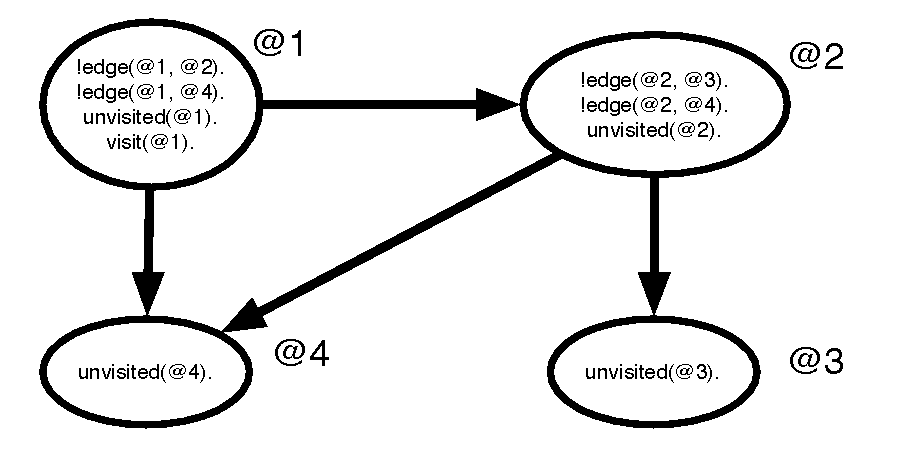
\includegraphics[width=\textwidth]{execution_trace1}
                \caption{Initial database.}
                \label{fig:exec_trace1}
        \end{subfigure}%
        ~ %add desired spacing between images, e. g. ~, \quad, \qquad etc.
          %(or a blank line to force the subfigure onto a new line)
        \begin{subfigure}[b]{0.5\textwidth}
                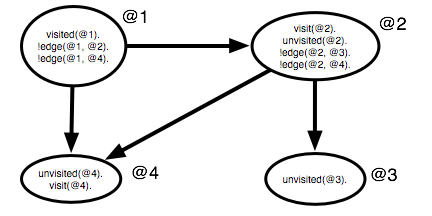
\includegraphics[width=\textwidth]{execution_trace2}
                \caption{After applying rule 1 at node $@1$.}
                \label{fig:exec_trace2}
        \end{subfigure}\\
        \begin{subfigure}[b]{0.5\textwidth}
                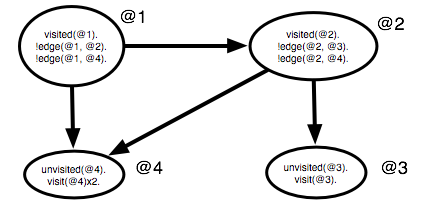
\includegraphics[width=\textwidth]{execution_trace3}
                \caption{After applying rule 1 at node $@2$.}
                \label{fig:exec_trace3}
        \end{subfigure}%
        ~ %add desired spacing between images, e. g. ~, \quad, \qquad etc.
         %(or a blank line to force the subfigure onto a new line)
        \begin{subfigure}[b]{0.5\textwidth}
                  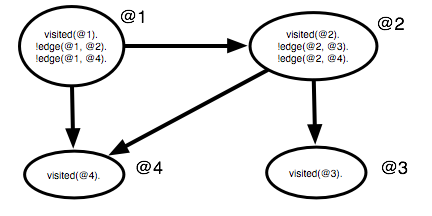
\includegraphics[width=\textwidth]{execution_trace4}
                  \caption{After applying rule 1 and 2 (nodes $@3$, $@4$).}
                  \label{fig:exec_trace4}
          \end{subfigure}
        \caption{One execution trace for the visit program.}\label{fig:exec_trace}
\end{figure}

Note that every node is now \texttt{visited}. It is easy to prove that if the graph is
connected, then all the nodes will be \texttt{visited}, regardless the order in which we
apply the rules.

\section{Syntax}

\renewcommand{\arraystretch}{1.5}


\begin{table}[ht]
   \centering
\begin{tabular}{ l l c l }
  Linear Facts & $L$ & $::=$ & $l(\hat{x})$\\
  Persistent Facts & $P$ & $::=$ & $\bang p(\hat{x})$\\
  Constraints & $C$ & $::=$ & $c(\hat{x})$ \\
  Action Facts & $A$ & $::=$ & $a(\hat{x})$\\
  Sensing Facts & $S$ & $::=$ & $s(\hat{x})$\\
  Body Expressions & $BE$ & $::=$ & $L \; | \; P \; | \; C \; | \; BE, BE \; | \; \forall_{\widehat{x}}. BE \; | \; \exists_{\widehat{x}}. BE \; | \; 1$\\
  Comprehensions & $CE$ & $::=$ & $\{ \; \widehat{x} \; | \; BE \; | \; CE \; \}$ \\
  Aggregates & $AE$ & $::=$ & $[\;\m{aop} \Rightarrow y \; | \; \widehat{x} \; | \; BE \; | \; HE \;]$ \\
  Exists constructor & $EE$ & $::=$ & $exists \; \widehat{x}. (HE)$ \\
  Head Expressions & $HE$ & $::=$ & $A \; | \; L \; | \; P \; | \; HE, HE \; | \; EE \; | \; CE \; | \; AE \; | \; 1$\\
  Rules & $R$ & $::=$ & $BE \lolli HE \; | \; [\; \m{sop} \Rightarrow y \; | \; BE \;] \lolli HE$ \\
  Set Of Rules & $\Sigma$ & $::=$ & $\cdot \; | \; \Sigma, R$\\
  Known Linear Facts & $\Delta$ & $::=$ & $\cdot \; | \; \Delta, l(\hat{t})$ \\
  Known Persistent Facts & $\Gamma$ & $::=$ & $\cdot \; | \; \Gamma, \bang p(\hat{t})$ \\
  Database & $D$ & $::=$ & $\Gamma; \Delta$ \\
\end{tabular}
\caption{Abstract syntax of \lang.}\label{tbl:ast}
\end{table}

\renewcommand{\arraystretch}{1.0}

Fig.~\ref{tbl:ast} shows the abstract syntax for derivation rules in \lang.
A \lang program consists of a set of derivation rules ($\Sigma$) and the database ($D$).
Each derivation can be decomposed into a body ($BE$) and a head ($HE$). An example of
a rule can be seen in line 11 in Fig.~\ref{code:visit}.
The body of this rule is \texttt{visit(A), visited(A)} and the head is \texttt{visited(A)}.
Rules without bodies are allowed in \lang and they are called axioms (line 15 in Fig.~\ref{code:visit}). Rules without heads are also allowed.

The body of the rule ($BE$) contains \emph{fact expressions} ($L$ and $P$) and
constraints ($C$). Fact expressions are template facts that instantiate variables
(from facts in the database)
such as \texttt{visit(A)} in line 11 in Fig.~\ref{code:visit}. Variables can be used again in the body for matching and
also in the head when instantiating facts. Constraints are boolean expressions that must
be true in order for the rule to be fired. Constraints use variables from fact expressions and are built using a small functional language that includes mathematical operations, boolean operations, external functions and literal values.

The head of a rule ($HE$) contains \emph{fact templates} ($L$ and $P$) which are uninstantiated facts and will derive new facts. The head can also have \emph{exist constructs} ($EE$), \emph{comprehensions} ($CE$) and \emph{aggregates} ($AE$). All those constructs
may use all the variables instantiated in the body.

\subsection{Predicates and Facts}

Each fact is an association between a \emph{predicate} and a tuple of values. A predicate is a pair with a name and a tuple of types (the argument types). \lang rules are type-checked using the predicate declarations in the header of the program. \lang has a simple type system that includes the following simples types: \emph{node}, \emph{int}, \emph{float}, \emph{string}, \emph{bool}. Recursive types such as \emph{list X} and \emph{pair X; Y} are
also allowed.

\subsection{Comprehensions}


Comprehensions ($CE$) are sub-rules that are applied with all possible combinations using the facts from the database. In a comprehension $\{ \; \widehat{x} \; | \; BE \; | \; CE \; \}$,
$\widehat{x}$ is the list of variables used inside $BE$ and $CE$. $BE$ and $CE$ are the
body and head of the comprehensions, respectively.

We have already seen an example of comprehensions in the visit program (Fig.~\ref{code:visit} line 9).
Here, we match \texttt{!edge(A, B)} using all the combinations
available in the database and for each combination we derive \texttt{visit(B)}.

\subsection{Aggregates}

Aggregates ($AE$) are a special kind of sub-rule that work very similarly to comprehensions.
In the abstract syntax $[\;\m{aop} \Rightarrow y \; | \; \widehat{x} \; | \; BE \; |
\; HE \;]$, $\m{aop}$ is the aggregate operation, $\widehat{x}$ are the variables
introduced in $BE$ and $HE$ and $y$ is the variable that is used inside the body
of the aggregate $BE$ and will be accumulated using $\m{aop}$. Like the comprehensions,
we try all the combinations of $BE$, but, instead of deriving $HE$ for each combination,
we accumulate the $y$ variable and derive $HE$ only once using $y$.

To better understand aggregates, let's consider a database with facts
\texttt{price(@1,~3)}, \texttt{price(@1,~4)}, \texttt{price(@1,~5)} and
\texttt{count-prices(@1)}. Now, consider the following rule:

\begin{Verbatim}
   count-prices(A) -o [:sum => P | | price(A, P) | total(A, P)].
\end{Verbatim}

By applying this rule, we consume \texttt{count-prices(@1)} and need to
derive the aggregate. The aggregate will consume all the \texttt{price(@1, P)} facts
and sum all the $P$'s. Finally, we derive \texttt{total(@1, 12)} since \texttt{P = 12}.

\lang provides several aggregate operations, including the minimum, maximum, sum, count, etc.

\subsection{Selectors}

When a rule body is instantiated using facts from the database, facts are picked
non-deterministically. While our system uses an implementation dependent order for
efficiency reasons, sometimes it is important to sort facts by one of the arguments
because linearity imposes commitment during rule derivation. The abstract syntax for
this construct is $[\; \m{sop} \Rightarrow y \; | \; BE \;] \lolli HE$, where
$\m{sop}$ is the selector operation, $BE$ the body of the rule where variable $y$
must be instantiated in the body of some fact and $HE$ is the head of the rule.
An example using concrete syntax is as follows:

\begin{Verbatim}
[:min => W | !edge(A, B), weight(A, B, W)] -o edge-picked(A, B, W).
\end{Verbatim}

In this case, we will order the \texttt{weight} facts by $W$ in ascending order and then try
to match them. Other operations available are $max$ and $random$ (to force randomization at the
implementation level).

\subsection{Exists Constructors}

Exist constructs ($EE$) are based on the linear logic construct of the same name and are used to create new node addresses. Although implicitly we use the exists connective inside the body
of the rule to instantiate variables from the database facts, in the head of the rule,
it can be used explicitly to create new variables.   
The following example illustrates the use of the exists constructor, where we derive
\texttt{perform-work} at a new node \texttt{B}.

\begin{Verbatim}
   do-work(A, W) -o exists B. (perform-work(B, W)).
\end{Verbatim}

\section{Types of Facts}

Beyond the distinction between linear and persistent facts, \lang further classifies facts
into 4 categories: computation facts, structural facts, sensing facts and action facts.

Computation facts are regular facts used to represent the program state. In the initial
example in Fig.~\ref{code:visit}, \texttt{visit}, \texttt{visited} and \texttt{unvisited}
are all computation facts.

Structural facts describe information about the connections between the nodes in the graph.
In the example of Fig.~\ref{code:visit}, the \texttt{edge} fact is structural since it
is marked as a \texttt{route} predicate. Note that structural facts can be seen as
computation facts since they also participate heavily in the program algorithm.

Sensing facts are facts about the current state of the runtime system, such as the placement
of nodes in the CPU and scheduling information. In the original Meld, sensing facts
were used to get information about the outside world, like temperature, touch data,
neighborhood status, etc.

Action facts are linear facts which are consumed when the corresponding action is performed.
In the original Meld, they were used to make the robots perform actions in the outside world.
For \lang we use them to change information about the program state
in the user interface. For example, when we want to change the color of nodes or the label
of edges, we just derive a new action fact and the action is performed in the interface.
A more important use of action facts is to change the order in which nodes
are evaluated in the runtime system. It is possible to give hints to the virtual
machine in order to prioritize the computation of some nodes.

With sensing facts and action facts, we can write "meta-rules" that will sense the
state of the runtime system and then apply decisions in order to improve execution speed.
In some situations, this set of rules can be added to the program without any modifications
to the original rules.

%%% Starts here



\section{Linearity}

\lang differs greatly from other Datalog-like languages due to the use of linear logic~\cite{Girard95logic:its}. Traditional forward-chaining logic programming languages make only use of classical logic, in which derived facts are true forever. Many ad-hoc extensions~\cite{Liu98extendingdatalog,Ludascher95alogical} have been devised in the past to support state updates in Datalog, but most are extra-logical which makes it harder to reason about programs.

We use a small subset of the original linear logic proof system with some extensions to improve
the expressiveness of the language. We summarize the connectives used in Table~\ref{table:linear}.

\begin{table*}
   \begin{center}
\resizebox{17cm}{!}{
    \begin{tabular}{ | l | l | l | l | l |}
    \hline
    Connective & Place & \lang Syntax & \lang Example & Description \\ \hline \hline
    $\emph{fact}(\hat{x})$ & Body or Head & $fact(\hat{x})$ & \texttt{path(A, P)} & Linear facts. \\ \hline
    $\bang \emph{fact}(\hat{x})$ & Body or Head & $\bang fact(\hat{x})$ & \texttt{$\bang$edge(X, Y, W)} & Persistent facts. \\ \hline
    $1$ & Head & $1$ & \texttt{1} & Represents rules with an empty head. \\ \hline
    $A \otimes B$ & Body and Head & $A, B$ & \texttt{path(A, P), edge(A, B, W)} & Connect two expressions. \\ \hline
    $\forall x. A$ & Rule & Please see $A \lolli B$ & \texttt{path(A, B) $\lolli$ reachable(A, B)} & To represent variables defined inside the rule. \\ \hline
    $\exists x. A$ & Head & $exists \; \widehat{x}. (B)$ & \texttt{exists A.(path(A, P))} & Instantiates new node variables. \\ \hline
    $A \lolli B$ & Rule & $A \lolli B$ & \texttt{path(A, B) $\lolli$ reachable(A, B)} & $\lolli$ means "linearly implies". \\& & & & $A$ is the body and $B$ is the head. \\ \hline
    $\m{def} A. B$ & Head & $\{\widehat{x} | A | B\}$ & \texttt{\{B | !edge(A, B) | visit(B)\}} & Extension called definitions.\\ & & & & Used for comprehensions and aggregates. \\ \hline
    \end{tabular}
}
\end{center}
\caption{Connectives from Linear Logic used in \lang.}
\label{table:linear}
\end{table*}

\section{Distribution}

The first argument of every predicate must be typed as a \emph{node}. The node represents a vertex in the graph data structure.
Essentially, a program can be seen as a graph data structure where processors do computation at the node/vertex level. Computation is
parallelized by processing many nodes concurrently. With the use of structural facts, it is
nodes are linked and can exchange facts between them.

For distribution and data partitioning purposes, derivation rules are constrained by the expressions that can be written in the body.
The body of every rule can only refer to facts in the same node.
However, the expressions in the head may refer to other nodes, as long as those nodes are instantiated in the body of the rule.
The database of the program is then partitioned by the first argument of each fact. This is possible since the rules of the
program only make use of facts from a single node.
We drew some inspiration from the Linda system~\cite{1663305}, where the tuple space contains the data and is used by the processors
to communicate and do computation.
This differs from imperative languages, since in those languages data and computation are two separate entities.

\section{Operational Semantics}

The execution is performed at the node level and can happen non-deterministically (i.e., any node can
be picked to run). This means that the programmer cannot expect
that facts coming from other nodes will be considered as a whole or partially.
Usually, it is preferable that rules are written as if rule order didn't matter, although
rule order makes things easier for ordering local computation.

Each rule in \lang has a defined priority that is inferred from its position in the source file.
Rules at the beginning of the file have higher priority. At the node level, we consider all
the new facts that have been not consider before in order to create a set of \emph{candidate rules}.
The set of candidate rules is then applied (by priority) and updated as new facts are derived or consumed.
Section~\ref{sec:core_engine} gives details in how our implementation manages the set of candidate rules.

\section{Programs}

In this section, we present several \lang programs in order to show that they tend to be concise and
easy to write. We also want to make clear how the language facilities can be used to solve more
complicated algorithms, including the quick-sort algorithm that at the first glance does not seem
to fit in the \lang paradigm.

\subsection{Quick-Sort}

The quick-sort algorithm is a divide and conquer sorting algorithm that works by splitting
a list of items into two sublists and then recursively sorting the two sublists.
To split the list, we pick a pivot element and put the items that are smaller than the pivot
into the first sublist and items greater than the pivot into the second list.

The quick-sort algorithm is interesting because it does not map immediately to the graph-based
model of \lang. Our approach considers that the program starts with a single node where
the initial list is located. Then we split the list as usual and create two nodes
that will recursively sort the sublists. Interestingly, this will create a tree
that will look similar to a call tree in a functional language.

Fig.~\ref{code:quicksort} presents the code for the quick-sort algorithm in \lang.
For each sublist to sort, we start with a \texttt{down} fact that must be (eventually)
transformed into an \texttt{up} fact, where the sublist in the \texttt{up} fact is sorted.
In line 12 we start with the initial list at node \texttt{@0}. Lines 14-17 will immediately
sort the list when the number of items is very small. Otherwise, we apply the rule in line 18.
\texttt{buildpivot} will first split the list using the pivot \texttt{X} using rules in
lines 24-27. When there is nothing more to split, we apply the rule in lines 20-23
that uses an exist constructor create nodes \texttt{B} and \texttt{C}. The sublists
are then sent to these nodes using \texttt{down} facts. Note, however, that we also
derive \texttt{back} facts, that will be used to send the sorted list back using the rule
in line 41.

When the sublists are finally sorted, we get two \texttt{sorted} facts that will match
against \texttt{waitpivot} in the rule located in lines 29-32. The sorted sublists
are appended and then an \texttt{up} fact is finally derived (line 38).

\begin{figure}[h!]
\small\begin{Verbatim}[numbers=left]
type linear route edge(node, node).
type route back(node, node).
type linear down(node, list int).
type linear up(node, list int).
type linear sorted(node, node, list int).
type linear buildpivot(node, list int, int, list int, list int).
type linear waitpivot(node, node, node, int).
type linear append(node, list int, list int).
type linear reverse(node, list int, list int, list int).
type linear reverse2(node, list int, list int).

down(@0, tosort).

down(A, []) -o up(A, []).
down(A, [X]) -o up(A, [X]).
down(A, [X, Y]), X < Y -o up(A, [X, Y]).
down(A, [X, Y]), X >= Y -o up(A, [Y, X]).
down(A, [X | L]) -o buildpivot(A, L, X, [], []).

buildpivot(A, [], X, Smaller, Greater)
   -o exists B, C. (back(B, A), down(B, Smaller),
            back(C, A), down(C, Greater), waitpivot(A, B, C, X)).

buildpivot(A, [Y | L], X, Smaller, Greater), Y <= X
   -o buildpivot(A, L, X, [Y | Smaller], Greater).
buildpivot(A, [Y | L], X, Smaller, Greater), Y > X
   -o buildpivot(A, L, X, Smaller, [Y | Greater]).
   
waitpivot(A, NodeSmaller, NodeGreater, Pivot),
sorted(A, NodeSmaller, Smaller),
sorted(A, NodeGreater, Greater)
   -o append(A, Smaller, [Pivot | Greater]).

append(A, L1, L2) -o reverse(A, L1, L2, []).

reverse(A, [], L2, L3) -o reverse2(A, L3, L2).
reverse(A, [X | L], L2, L3) -o reverse(A, L, L2, [X | L3]).
reverse2(A, [], Result) -o up(A, Result).
reverse2(A, [X | L1], L2) -o reverse2(A, L1, [X | L2]).

up(A, L), back(A, B) -o sorted(B, A, L).
\end{Verbatim}
  \caption{Quick-Sort program.}
  \label{code:quicksort}
\end{figure}
\normalsize

\subsection{Bipartiteness Checking}

The problem of checking if a graph is bipartite can be seen as a 2-color graph coloring problem.
The code for this algorithm is shown in Fig.~\ref{code:bichecking}. All nodes in the graph
start as \texttt{unchecked}, because they do not have a color yet. The axiom \texttt{visit(@1, 1)} is
instantiated at node \texttt{@1} (line 9) in order to color this node with color 1.

If a node is \texttt{unchecked} and needs to be marked with a color \texttt{P} then the rule in
lines 11-12 is applied. We consume the \texttt{unchecked} fact and derive a \texttt{checked(A, P)}
to effectively color the node with \texttt{P}. We also derive \texttt{visit(B, next(P))} in
our neighbor nodes in order to color them with the other color.

The coloring can fail is the node is already colored and a color \texttt{P} and needs to be colored
with a different color (line 14) or if it has already failed (line 16).

\begin{figure}[h!]
\small\begin{Verbatim}[numbers=left]
type route edge(node, node).
type linear visit(node, int).
type linear unchecked(node).
type linear checked(node, int).
type linear fail(node).

fun next(int X) : int = if X <> 1 then 1 else 2 end.

visit(@1, 1).

visit(A, P), unchecked(A)
   -o {B | !edge(A, B) | visit(B, next(P))}, checked(A, P).

visit(A, P1), checked(A, P2), P1 <> P2 -o fail(A).
visit(A, P), checked(A, P) -o checked(A, P).
visit(A, P), fail(A) -o fail(A).
\end{Verbatim}
  \caption{Bipartiteness Checking program.}
  \label{code:bichecking}
\end{figure}
\normalsize

\subsection{N Queens}


The N queens~\cite{8queens} puzzle is the problem of placing N chess queens on an NxN chessboard so
that no pair of two queens attack each other. The specific challenge of finding all the distinct
solutions to this problem is a good benchmark in designing parallel algorithms.

First, we consider each square of the chessboard as a node
that can communicate with the adjacent left, right and bottom squares, but not top square.
The states are represented as a list of integers, where each integer is the column number where
the queen was placed. For example $[2, 0]$ means that a queen was placed in $(0, 0)$ and $(1, 2)$.

An empty state is instantiated in the top-left node and is then propagated to all nodes in the same row.
Every node will then check if a queen can be placed on the square. If true, each node will send the new
state to the row below.
Recursively, when a node receives a new state, it will (1) send the state to the left
and to the right and (2) try to place the queen in its square. With this method,
all states will be computed since we have facts for each valid state
at that point. When a square cannot place a queen, that state is deleted.
When the program ends, the states will be placed in the bottom row.

We find our solution very elegant, since it can be easily executed in parallel and there are no
wasted computations, because any distinct placement will be computed only once.

\begin{comment}
\begin{figure}[h!]
\small\begin{Verbatim}[numbers=left]
type left(node, node).
type right(node, node).
type down(node, node).
type coord(node, int, int).
type linear propagate-left(node, list node, list int).
type linear propagate-right(node, list node, list int).
type linear receive-down(node, list node, list int).
type linear test-and-send-down(node, list node, list int).
type linear test-y(node, int, list int, list node, list int).
type linear test-diag-left(node, int, int, list int, list node, list int).
type linear test-diag-right(node, int, int, list int, list node, list int).
type linear send-down(node, list node, list int).
type linear final-state(node, list node, list int).

const size = 11.

receive-down(@0, [], []).

receive-down(A, Nodes, Coords)
   -o {R | !right(A, R), R <> A | propagate-right(R, Nodes, Coords)},
      {L | !left(A, L), L <> A | propagate-left(L, Nodes, Coords)},
      test-and-send-down(A, Nodes, Coords).

propagate-left(A, Nodes, Coords)
   -o {L | !left(A, L), L <> A | propagate-left(L, Nodes, Coords)},
      test-and-send-down(A, Nodes, Coords).

propagate-right(A, Nodes, Coords)
   -o {R | !right(A, R), R <> A | propagate-right(R, Nodes, Coords)},
      test-and-send-down(A, Nodes, Coords).

test-and-send-down(A, Nodes, Coords),
!coord(A, X, Y)
   -o test-y(A, Y, Coords, Nodes, Coords).

test-y(A, Y, [], Nodes, Coords), !coord(A, OX, OY) -o test-diag-left(A, OX - 1, OY - 1, Coords, Nodes, Coords).
test-y(A, Y, [X, Y1 | RestCoords], Nodes, Coords), Y = Y1 -o 1. // fail
test-y(A, Y, [X, Y1 | RestCoords], Nodes, Coords), Y <> Y1 -o test-y(A, Y, RestCoords, Nodes, Coords).

test-diag-left(A, X, Y, _, Nodes, Coords),
X < 0 || Y < 0,
!coord(A, OX, OY)
   -o test-diag-right(A, OX - 1, OY + 1, Coords, Nodes, Coords).

test-diag-left(A, X, Y, [X1, Y1 | RestCoords], Nodes, Coords),
X = X1, Y = Y1
   -o 1. // fail

test-diag-left(A, X, Y, [X1, Y1 | RestCoords], Nodes, Coords),
X <> X1 || Y <> Y1
   -o test-diag-left(A, X - 1, Y - 1, RestCoords, Nodes, Coords).

test-diag-right(A, X, Y, [], Nodes, Coords),
X < 0 || Y >= size,
!coord(A, OX, OY)
   -o send-down(A, [A | Nodes], [OX, OY | Coords]).

test-diag-right(A, X, Y, [X1, Y1 | RestCoords], Nodes, Coords),
X = X1, Y = Y1
   -o 1. // fail

test-diag-right(A, X, Y, [X1, Y1 | RestCoords], Nodes, Coords),
X <> X1 || Y <> Y1
   -o test-diag-right(A, X - 1, Y + 1, RestCoords, Nodes, Coords).

send-down(A, Nodes, Coords),
!down(A, A)
   -o final-state(A, Nodes, Coords).
   
send-down(A, Nodes, Coords),
!down(A, B),
A <> B
   -o receive-down(B, Nodes, Coords).
\end{Verbatim}
  \caption{Visit program.}
  \label{code:visit}
\end{figure}
\normalsize
\end{comment}

\section{Summary}

In this chapter we gave an overview of the \lang language, including its syntax and operational semantics.
We also explained how to write programs using all the facilities provided by \lang, including
linear facts and comprehensions. Since \lang uses implicit parallelism, programs can be run in parallel
in multicore architectures without any modification.

\chapter{Coordination}
The original Meld was
implemented as an ensemble programming language, targeting modular robotic systems such as
Claytronics~\cite{ashley-rollman-derosa-iros07wksp}. In such systems, there is a natural matching
between computation and processing units, since each robot is represented by a node. This distribution
of data leaves little choice to be made in the division of computation to the various nodes.

On the other hand, \lang has no natural matching of data and computation to workers (processes, threads),
since nodes are a program abstraction and part of the program's logic.
We view the set of nodes as a graph data structure where workers will perform work.
A worker is able to process any node, although a node cannot be computed by more than one worker
at the same time. This disallows the manipulation of a node by multiple workers.

Since \lang uses linear logic, the order in which nodes are scheduled can impact the
performance and even the results of the program. When only using
classical logic, no matter how computation is done, the end result will be the same since the program
is strictly monotonic.
\lang introduces the concept of \emph{coordination} that allows the programmer
to write code that changes how the runtime system schedules nodes.

Randomized and approximation
algorithms can obtain significant benefits from coordination directives because although the final
program results will not be exact, they follow important statistical properties and can be computed faster.
Examples of such programs are PageRank~\cite{Lubachevsky:1986:CAA:4904.4801} and
Loopy Belief Propagation~\cite{Gonzalez+al:aistats09paraml}.

\section{Scheduling Facts}

We can use action facts to change the order in which nodes are evaluated by adding
\emph{priorities}. Node priority works at the worker level
so that each worker can make a local decision about which node of the graph to run next.
Note that, by default, nodes are picked arbitrarily (a FIFO approach is used).

The following list presents the action facts available to manipulate the scheduling decisions of the system:

\begin{description}
   \item[\texttt{type linear action set-priority(node, float)}]: This sets the priority of a node. If the node already has some priority, we only change the priority if the new one is higher priority. The programmer can decide if priorities are to be ordered in ascending or descending order.
   \item[\texttt{type linear action add-priority(node, float)}]: This gets the current node's priority and increases or decreases it.
   \item[\texttt{type linear action schedule-next(node)}]: The work will fetch the highest priority node's priority $P$ from its set of nodes and set the action's argument node's priority as $P + 1.0$. If using the priorities
   in ascending order, we pick the lowest priority and subtract $1.0$.
   \item[\texttt{type linear action unset-priority(node)}]: Removes the priority, if any, of a given node.
   \item[\texttt{type linear action stop-program(node)}]: Immediately stops the execution of the whole program.
\end{description}

When the highest priority node is picked up for execution, its priority is reset to 0 (the default priority value). This means that
the programmer must set the node's priority again if he wants to prioritize that node.

We intend to add more action facts in the near future. For example, we want the programmer to be able to place specific nodes in workers. This will permit good use of
memory locality by forcing certain computations to be performed in the same worker.

Sensing facts provide information about node placement and node priority. We can use those facts
to express coordination policies. \lang provides the following two
sensing facts:

\begin{description}
   \item[\texttt{type linear cpu-id(node, node, int).}] The third argument indicates the worker's ID where the node of the second argument is currently running.
   \item[\texttt{type linear priority(node, node, float).}] The third argument is the current priority of the node in the second argument.
\end{description}

Note that when sensing facts are consumed, they are re-derived automatically, except if the programmer explicitly tells the compiler otherwise. 

\subsection{Global Directives}

We also provide a few global coordination statements:

\begin{description}
   \item[\texttt{priority @order ORDER.}] \texttt{ORDER} can be either \texttt{asc} or \texttt{desc}. This defines if node's are to be selected by the smallest or the greatest priority, respectively.
   \item[\texttt{priority @initial P.}] The \texttt{initial} statement informs the runtime system that all nodes must start with priority $P$. Alternatively, the programmer can define an \texttt{set-priority(A, P)} axiom.
   \item[\texttt{priority @static.}] The \texttt{static} priority tells the runtime system that the partition of nodes among workers is to be used until the end of program. 
   %\item[\texttt{priority @cluster TYPE.}] Define what type of graph clustering to use. \texttt{TYPE} can be either \texttt{static}, \texttt{bfs} or \texttt{random}.
\end{description}

\section{Programs}

To better understand how coordination directives work, we next present some programs that
take advantage of them.

\subsection{Single Source Shortest Path}

The Single Source Shortest Path (SSSP) is a graph algorithm where we want to compute the
distance of all nodes to a single node. The full code is presented in Fig.~\ref{code:shortest_path_program}.
The graph is represented using the \texttt{edge(A,~B,~W)} predicate (line 1), where
\texttt{A} $\rightarrow$ \texttt{B} is a directed edge from node \texttt{A} to \texttt{B}
with distance \texttt{W}. The second predicate is \texttt{path(A,~D,~F)} (line 2), where
\texttt{D} is the distance of node \texttt{A} to our initial node and \texttt{F}
indicates if this path has been processed.

Every node may have several \texttt{path} facts. From this set of facts, the node will select
the path with the least distance (rules in lines 11-13) and then propagate it using the third rule (lines 15-19).
When a path is used for propagation, we make sure that the path flag is \texttt{notused} (line 15)
because we do not want to propagate the same distance twice. When the rule is fired, the flag
then changes to \texttt{used} (line 19).

We start with the axiom \texttt{path(startnode,~0,~notused)} in line 9 (the distance to the starting
node is \texttt{0}). This will kickstart the computation by propagating the initial distance to the
neighbor nodes using rule 3. We also use 2 coordination directives:

\begin{itemize}
   \item \texttt{priority~@order~asc}: paths are picked in ascending order (line 4).
   \item \texttt{set-priority(B,~D~+~W)}: to change the node's priority upon the computation of
a new distance (line 18).
\end{itemize}

With these directives, we ensure that we pick the node with the smallest distance
first. If we are only using 1 thread, then our algorithm will behave like Dijkstra's shortest
path algorithm~\cite{Dijkstra}. When using more than 1 thread, each thread will pick the smallest
path from a subset of nodes. This is an example where using coordination directives will
improve the speed of execution since we avoid propagating some of the paths.

\begin{figure}[h!]
\small\begin{Verbatim}[numbers=left,commandchars=&\[\]]
type route edge(node, node, int).
type linear path(node, int, int).

&underline[priority @order asc].

const visited = 1.
const notused = 0.

path(startnode, 0, notused).

path(A, B, used), path(A, B, notused) -o path(A, B, used).

path(A, B1, X), path(A, B2, Y), B1 <= B2 -o path(A, B1, X).

path(A, D, notused)
   -o {B, W | !edge(A, B, W) |
         path(B, D + W, notused),
         &underline[set-priority(B, D + W))]},
      path(A, D, used).
\end{Verbatim}
  \caption{Shortest Path Program.}
  \label{code:shortest_path_program}
\end{figure}
\normalsize
\subsection{Splash BP}

Loopy Belief Propagation~\cite{Murphy99loopybelief} (LBP) is an approximate inference algorithm
used in graphical models with cycles. In its essence, LBP is a sum-product message passing algorithm
where nodes exchange messages with their immediate neighbors and apply some computations to the messages
received.

LBP is an algorithm that maps very well to the graph based model of LM. In its original form, we need to compute
the belief of all nodes for several iterations and also synchronize after each iteration.
However, it is still possible to apply
some optimizations in order to take advantage of the fact that LBP will converge even when using
an asynchronous approach. So, instead of computing the belief iteratively,
we first keep track of all messages sent/received (and overwrite them when we receive a new one)
and recompute the belief when we want, instead of synchronizing between nodes.
This way, we can prioritize the computation of beliefs when
a node's belief value changes significantly. When that happens, we set the priority of its
neighbors so that they can recompute their beliefs.

The asynchronous approach proves to be a nice improvement over the synchronous version. Still, it
is possible to do even better. Gonzalez et al~\cite{Gonzalez+al:aistats09paraml} developed an optimal
algorithm to compute this algorithm by first building a tree and then updating the beliefs of each node twice, first from the leaves to the root and then from the root to the leaves. The root of this tree
is the node with the highest priority (based on belief) while the other nodes in the tree
must have a non-zero priority. Note that the priorities are updated whenever a neighbor updates
their belief. These splash trees are built iteratively until we reach convergence.

The code in Fig.~\ref{code:sbp} presents the coordination code of the Belief Propagation problem.
Please note that we just appended the code in Fig.~\ref{code:sbp} to a working but
unoptimized version of the algorithm.
In the coordination code we have three sections:
\begin{description}
   \item[Tree building]: Each node has a \texttt{waiting} fact that is used to start the tree building process. When the highest priority is picked we create a token that will navigate through the tree. Note that in the rule located in lines 11-18 we check if the priority of the new node to add to the tree is positive and that both nodes are in the same worker. We want the tree to be kept in the same worker.
   \item[First phase]: In the third rule (lines 8-9), when we reach a certain number of nodes in the tree, we generate \texttt{first-phase} in order to update the beliefs of all nodes in tree starting from the leaves and ending at the root. As we update the nodes, we generate \texttt{update} to update the belief values (line 29).
   \item[Second phase]: In the second phase we go from the root to the leaves and update the beliefs a second time (line 39).
\end{description}

When we have several workers, every worker will generate their own trees by taking into account the highest priority node in their own queues.

\begin{figure}[h!]
\small\begin{Verbatim}[numbers=left,commandchars=*\{\}]
// TREE BUILDING
// continue tree
waiting(A), token(A, All, Next) -o token(A, All, Next).
// start tree
waiting(A), *underline{@priority(A, A, P)}, P > 0.0
   -o token(A, [A], [A]).
// end tree building
token(A, All, Next), length(All) > maxnodes
   -o first-phase(A, All, reverse(All)).
// expand tree
token(A, All, [A | Next])
   -o [collect => L | Side | !edge(A, L, Side),
         0 = count(All, L),
         0 = count(Next, L),
         *underline{priority(A, L, P)}, P > 0.0,
         *underline{cpu-id(A, L, Id1)},
         *underline{cpu-id(A, A, Id2)}, Id1 = Id2 |
         send-token(A, All, Next ++ L)].

send-token(A, All, [])
   -o first-phase(A, All, reverse(All)).
send-token(A, All, [B | Next])
   -o *underline{schedule-next(B)},
      token(B, All ++ [B], [B | Next]).

// FIRST PHASE
first-phase(A, [A], [A]) -o second-phase(A, [], A).
first-phase(A, [A, B | Next], [A])
   -o update(A), *underline{schedule-next(B)},
      second-phase(B, [B | Next], A).
first-phase(A, All, [A, B | Next])
   -o update(A), *underline{schedule-next(B)},
      first-phase(B, All, [B | Next]).

// SECOND PHASE
second-phase(A, [], _)
   -o *underline{set-priority(A, 0.0)}, waiting(A), update(A).
second-phase(A, [A], Back)
   -o update(A), waiting(Back),
      waiting(A), *underline{set-priority(A, 0.0)}.
second-phase(A, [A, B | Next], Back)
   -o update(A), waiting(Back), *underline{schedule-next(B)},
      second-phase(B, [B | Next], A).
\end{Verbatim}
  \caption{Coordination code for the Splash Belief Propagation program.}
  \label{code:sbp}
\end{figure}
\normalsize

\section{Summary}

In this chapter we presented the current set of coordination directives, implemented as sensing and action facts. The use of such facilities allows the programmer to write derivation rules that change how
the runtime system schedules computation thus improving the executing time and possibly the final program
results. As future work, we intend to extend the set of available directives and write additional programs using coordination.


\chapter{Proof Theoretic Semantics}
\newcommand{\mz}{\m{match} \;}
\newcommand{\tab}[0]{\;\;\;\;}
\newcommand{\dz}{\m{derive} \;}
\newcommand{\comp}[0]{\m{comp} \;}
\newcommand{\az}{\m{apply} \;}
\newcommand{\doz}{\m{run} \;}
\newcommand{\seqnocut}[3]{#1 ; #2 \Rightarrow #3}
\newcommand{\defeq}{\buildrel\triangle\over =}
\newcommand{\compr}[1]{\m{def} \; #1}

\newcommand{\mo}{\m{match}_1 \;}
\newcommand{\cont}{\m{cont} \;}
\newcommand{\contc}{\m{contc} \;}
\newcommand{\done}{\m{derive}_1 \;}
\newcommand{\doo}{\m{run}_1 \;}
\newcommand{\mc}[0]{\m{match}_c \; }
\newcommand{\dall}[0]{\m{fix} \; }
\newcommand{\strans}[0]{\m{strans} \;}
\newcommand{\dc}{\m{derive}_c \;}
\newcommand{\ao}{\m{apply}_1 \;}

This chapter provides a brief overview of the proof theoretic basis behind \lang and the dynamic semantics
of the language. First, we will present the subset of linear logic from which \lang is built on. Second, we present the high level dynamic semantics (how rules are evaluated) followed by the low level dynamics, a close representation of how to virtual machine runs. Finally, we give an overview of the soundness proof of the low level semantics.

\section{Linear Logic}

\lang differs greatly from other Datalog-like languages due to the use of linear logic~\cite{Girard95logic:its}. Traditional forward-chaining logic programming languages make only use of classical logic, in which derived facts are true forever. Many ad-hoc extensions~\cite{Liu98extendingdatalog,Ludascher95alogical} have been devised in the past to support state updates in Datalog, but most are extra-logical which makes it harder to reason about programs.
\lang uses linear logic as its foundation, therefore state updates are completely natural to the language.

We use a small subset of the original linear logic proof along with an extension for definitions to improve
the expressiveness of the language. We summarize the connectives used in Table~\ref{table:linear}
and how they are related to the \lang syntax.

\begin{table*}
   \begin{center}
\resizebox{16cm}{!}{
    \begin{tabular}{ | l | l | l | l | l |}
    \hline
    Connective & Place & \lang Syntax & \lang Example & Description \\ \hline \hline
    $\emph{fact}(\hat{x})$ & Body or Head & $fact(\hat{x})$ & \texttt{path(A, P)} & Linear facts. \\ \hline
    $\bang \emph{fact}(\hat{x})$ & Body or Head & $\bang fact(\hat{x})$ & \texttt{$\bang$edge(X, Y, W)} & Persistent facts. \\ \hline
    $1$ & Head & $1$ & \texttt{1} & Represents rules with an empty head. \\ \hline
    $A \otimes B$ & Body and Head & $A, B$ & \texttt{path(A, P), edge(A, B, W)} & Connect two expressions. \\ \hline
    $\forall x. A$ & Rule & Please see $A \lolli B$ & \texttt{path(A, B) $\lolli$ reachable(A, B)} & To represent variables defined inside the rule. \\ \hline
    $\exists x. A$ & Head & $exists \; \widehat{x}. (B)$ & \texttt{exists A.(path(A, P))} & Instantiates new node variables. \\ \hline
    $A \lolli B$ & Rule & $A \lolli B$ & \texttt{path(A, B) $\lolli$ reachable(A, B)} & $\lolli$ means "linearly implies". \\& & & & $A$ is the body and $B$ is the head. \\ \hline
    $\m{def} A. B$ & Head & $\{\; \widehat{x} \; | \; A \; | \; B \; \}$ & \texttt{\{B | !edge(A, B) | visit(B)\}} & Extension called definitions.\\ & & & & Used for comprehensions and aggregates. \\ \hline
    \end{tabular}
}
\end{center}
\caption{Connectives from Linear Logic used in \lang.}
\label{table:linear}
\end{table*}

The sequent calculus for our linear logic fragment is shown in Fig.~\ref{linear_logic}.
The sequent has the form $\Psi ; \seqnocut{\Gamma}{\Delta}{C}$, where $\Psi$ is the typed
term context used in the quantifiers, $\Gamma$ is the multi-set of persistent facts, $\Delta$
is the multi-set of linear facts and $C$ is the term we want to prove.

Most connectives in our fragment are standard and well known, except for the $\compr{A}$ connective. This
connective is a definition that can be unfolded recursively and is used to logically justify
comprehensions and aggregates. We took inspiration from Baelde's work on least and greatest fixed points
in linear logic~\cite{Baelde:2012:LGF:2071368.2071370}. Baelde's system goes beyond simple recursive
definitions and allows proofs using induction and co-induction proofs in linear logic. Fortunately,
the proof system satisfies cut-elimination which makes it consistent. 

In a comprehension, we want to imply an implication as many times as possible matches we can do
using the current database. One way to formally describe comprehensions would be to use persistent
rules that would be used a few times and then would be forgotten. A more reasonable approach is to use
definitions. Given a comprehension $C$ with a body $A$ and a head $B$, then we can build the following definition:

\[
\compr{C} \defeq 1 \with ((A \lolli B) \otimes \compr{C})
\]

We can unfold $\compr{C}$ to either stop (by selecting $1$) or get a new linear implication $A \lolli B$
to apply the comprehension once. Because we also get another $\compr{C}$ by selecting the right hand side,
the comprehension can be applied again, recursively.

Aggregates work identically, but they need an extra argument to accumulate the aggregated value.
If an aggregate $C$ uses the \texttt{sum} operation and has a body $B$ then the definition will be
as follows:

\[
\compr{C} \; V \defeq (\lambda v. B)V \with (\forall x. Ax \lolli \compr{C} \; (x + V))
\]

The aggregate is initiated as $\compr{C} \; 0$.

\begin{figure}[ht]
\[
\infer[\one R]
{\Psi ; \seqnocut{\Gamma}{\cdot}{\one}}
{}
\tab
\infer[\one L]
{\Psi ; \seqnocut{\Gamma}{\Delta, \one}{C}}
{\Psi ; \seqnocut{\Gamma}{\Delta}{C}}
\]

\[
\infer[\with R]
{\Psi ; \seqnocut{\Gamma}{\Delta}{A \with B}}
{\Psi ; \seqnocut{\Gamma}{\Delta}{A} & \seqnocut{\Gamma}{\Delta}{B}}
\tab
\infer[\with L_1]
{\Psi ; \seqnocut{\Gamma}{\Delta, A \with B}{C}}
{\Psi ; \seqnocut{\Gamma}{\Delta, A}{C}}
\tab
\infer[\with L_2]
{\Psi ; \seqnocut{\Gamma}{\Delta, B \with B}{C}}
{\Psi ; \seqnocut{\Gamma}{\Delta, B}{C}}
\]

\[
\infer[\otimes R]
{\Psi ; \seqnocut{\Gamma}{\Delta, \Delta'}{A \otimes B}}
{\Psi ; \seqnocut{\Gamma}{\Delta}{A} & \seqnocut{\Gamma}{\Delta}{B}}
\tab
\infer[\otimes L]
{\Psi ;\seqnocut{\Gamma}{\Delta, A \otimes B}{C}}
{\Psi ; \seqnocut{\Gamma}{\Delta, A, B}{C}}
\]

\[
\infer[\lolli R]
{\Psi ; \seqnocut{\Gamma}{\Delta}{A \lolli B}}
{\Psi ; \seqnocut{\Gamma}{\Delta, A}{B}}
\tab
\infer[\lolli L]
{\seqnocut{\Gamma}{\Delta, \Delta', A \lolli B}{C}}
{\Psi ; \seqnocut{\Gamma}{\Delta}{A} &
   \Psi ; \seqnocut{\Gamma}{\Delta', B}{C}}
\]

\[
\infer[\forall R]
{\Psi ; \seqnocut{\Gamma}{\Delta}{\forall n:\tau. A}}
{\Psi, m:\tau ; \seqnocut{\Gamma}{\Delta}{A\{m/n\}}}
\tab
\infer[\forall L]
{\Psi ; \seqnocut{\Gamma}{\Delta, \forall n:\tau. A}{C}}
{\Psi \vdash M : \tau & \Psi ; \seqnocut{\Gamma}{\Delta, A\{M/n\}}{C}}
\]

\[
\infer[\exists R]
{\Psi ; \seqnocut{\Gamma}{\Delta}{\exists n: \tau. A}}
{\Psi \vdash M : \tau &
   \Psi ; \seqnocut{\Gamma}{\Delta}{A \{M/n\}}}
\tab
\infer[\exists L]
{\Psi ; \seqnocut{\Gamma}{\Delta, \exists n:\tau. A}{C}}
{\Psi, m:\tau ; \seqnocut{\Gamma}{\Delta, A\{m/n\}}{C}}
\]

\[
\infer[\bang R]
{\Psi ; \seqnocut{\Gamma}{\cdot}{\bang A}}
{\Psi ; \seqnocut{\Gamma}{\cdot}{A}}
\tab
\infer[\bang L]
{\Psi ; \seqnocut{\Gamma}{\Delta, \bang A}{C}}
{\Psi ; \seqnocut{\Gamma, A}{\Delta}{C}}
\tab
\infer[\m{copy}]
{\Psi ; \seqnocut{\Gamma, A}{\Delta}{C}}
{\Psi ; \seqnocut{\Gamma, A}{\Delta, A}{C}}
\]

\[
\infer[\m{def} \; R]
{\Psi ; \seqnocut{\Gamma}{\Delta}{\compr{A'}}}
{\Psi ; \seqnocut{\Gamma}{\Delta}{B\theta} &
 A \defeq B & A' \doteq A\theta}
\tab
\infer[\m{def} \; L]
{\Psi ; \seqnocut{\Gamma}{\Delta, \compr{A'}}{C}}
{
   \Psi ; \seqnocut{\Gamma}{\Delta, B\theta}{C} & A \defeq B & A' \doteq A\theta
}
\]
\caption{Linear logic fragment used in \lang.}\label{linear_logic}
\end{figure}

\section{High Level Dynamic Semantics}

In this section, we are going to present the high level dynamic semantics of \lang. The semantics
formalize the mechanism of matching rules and deriving new facts. The high level semantics
present a simplified overview of the dynamics of the language that are more closer to the formalism
of linear logic present in Fig.~\ref{linear_logic} than the implementation principles of our
virtual machine.

Both the high level and low level semantics do not model the use of variable bindings when matching
facts from the database. The formalization of bindings tends to complicate the formal system and it is not
necessary for a good understanding of the system. Instead, we assume that all facts of
type $\emph{fact}(\hat{x})$ do not have the argument $\hat{x}$.

Starting from the linear logic fragment presented earlier, we consider $\Gamma$ and $\Delta$ the database
of our program. $\Gamma$ contains the database of persistent facts while $\Delta$ the database of linear
facts. We assume that the rules of the program are persistent linear implications of the form
$\bang (A \lolli B)$, that can be used several times. However, we do not put the rules in the $\Gamma$
context but in a separate context $\Phi$.

The main idea of the dynamic semantics is to mostly ignore the right side of the sequent calculus
and use inversion on the $\Delta$ and $\Gamma$ context so that we only have atomic facts.
To apply rules we use chaining by focusing on one of the derivation rules in $\Phi$. Note
that in the focusing process we assume that all the atoms (facts) are positive thus the chaining
becomes a forward chaining process.

\subsubsection{Application}

The main judgment of the system is $\doz \Gamma; \Delta; \Phi \rightarrow \Xi'; \Delta'; \Gamma'$.
$\Gamma$, $\Delta$ and $\Phi$ have the meaning explained before, while $\Xi'$, $\Delta'$ and $\Gamma'$
are output multi-sets from applying one of the rules in $\Phi$. $\Xi'$ is the set of consumed linear
resources, $\Delta'$ is the set of derived linear facts and $\Gamma'$ is the set of derived persistent
facts. Note that for the high level semantics there is no concept of rule priority, so we pick a rule
non-deterministically.

The judgment $\az \Gamma ; \Delta ; A \lolli B \rightarrow \Xi'; \Delta'; \Gamma'$ will attempt to apply
the derivation rule $A \lolli B$. To do this, it splits the $\Delta$ context into two, namely the
set of linear resources consumed to match the body of the rule and the remaining facts. Again the
set of resources needed to match the body of the rule is guessed. The low level dynamic semantics will
handle this.

\[
\infer[\az rule]
{\az \Gamma ; \Delta, \Delta'' ; A \lolli B \rightarrow \Xi' ; \Delta' ; \Gamma'}
{\mz \Gamma ; \Delta ; A \rightarrow \Delta & \dz \Gamma ; \Delta''; \Delta; \cdot ; \cdot ; B \rightarrow \Xi' ; \Delta' ; \Gamma'}
\]

\[
\infer[\doz rule]
{\doz \Gamma ; \Delta ; R, \Phi \rightarrow \Xi' ; \Delta' ; \Gamma'}
{\doz \Gamma ; \Delta ; R \rightarrow \Xi' ; \Delta' ; \Gamma'}
\]

\subsubsection{Match}

The $\mz \Gamma ; \Delta \rightarrow C$ judgment essentially uses the right rules of the original
linear logic fragment in order to match all facts using $\Gamma$ and $\Delta$.

\[
\infer[\mz 1]
{\mz \Gamma; \cdot \rightarrow 1}
{}
\tab
\infer[\mz p]
{\mz \Gamma; p \rightarrow p }
{}
\tab
\infer[\mz \bang p]
{\mz \Gamma, p; \cdot \rightarrow \bang p}
{}
\]

\[
\infer[\mz \otimes]
{\mz \Gamma; \Delta_1, \Delta_2 \rightarrow A \otimes B}
{\mz \Gamma; \Delta_1 \rightarrow A & \mz \Delta_2 \rightarrow B}
\]

\subsubsection{Derivation}

The derivation judgment has the form $\dz \Gamma ; \Delta ; \Xi ; \Gamma_1 ; \Delta_1 ; \Omega \rightarrow \Xi'; \Delta'; \Gamma'$ with the following meaning:

\begin{enumerate}
   \item[$\Gamma$] the multi-set of persistent resources in the database.
   \item[$\Delta$] the multi-set of linear resources in the database not yet consumed.
   \item[$\Xi$] the multi-set of linear resources that have been consumed while matching the body of the rule, matching comprehensions or aggregates.
   \item[$\Gamma_1$] the multi-set of persistent facts that have been derived using the current rule.
   \item[$\Delta_1$] the multi-set of linear facts that have been derived using the current rule.
   \item[$\Omega$] an ordered list contain the terms of the head of rule that still need to be derived. We start with the head of the rule $B$ that is continuously deconstructed to derive all the facts of the rule.
   \item[$\Xi'$] the consumed linear facts to apply this rule.
   \item[$\Delta'$] the derived linear facts.
   \item[$\Gamma'$] the derived persistent facts.
\end{enumerate}

We did not include the aggregates here because they are similar to comprehensions. The main rule to
derive comprehensions is $\dz comp$. It unfolds the comprehension which it can be then either
applied ($\dz \with R$ followed by $\dz \lolli$) or not ($\dz \with L$). The high level semantics
do not take into account the contents of the database to determine how many times a comprehension
should be applied because it is entirely non-deterministic.



\[
\infer[\dz p]
{\dz \Gamma ; \Delta ; \Xi ; \Gamma_1 ; \Delta_1 ; p, \Omega \rightarrow \Xi' ; \Delta' ; \Gamma'}
{\dz \Gamma ; \Delta ; \Xi ; \Gamma_1 ; p, \Delta_1 ; \Omega \rightarrow \Xi' ; \Delta' ; \Gamma'}
\]

\[
\infer[\dz \bang p]
{\dz \Gamma ; \Delta ; \Xi ; \Gamma_1 ; \Delta_1 ; \bang p, \Omega \rightarrow \Xi' ; \Delta' ; \Gamma'}
{\dz \Gamma ; \Delta ; \Xi ; \Gamma_1, p ; \Delta_1 ; \Omega \rightarrow \Xi' ; \Delta' ; \Gamma'}
\]

\[
\infer[\dz \otimes]
{\dz \Gamma ; \Delta ; \Xi ; \Gamma_1 ; \Delta_1 ; A \otimes B, \Omega \rightarrow \Xi' ; \Delta' ; \Gamma'}
{\dz \Gamma ; \Delta ; \Xi ; \Gamma_1 ; \Delta_1 ; A, B, \Omega \rightarrow \Xi' ; \Delta' ; \Gamma'}
\]

\[
\infer[\dz 1]
{\dz \Gamma ; \Delta ; \Xi ; \Gamma_1; \Delta_1 ; 1, \Omega \rightarrow \Xi' ; \Delta' ; \Gamma'}
{\dz \Gamma ; \Delta ; \Xi ; \Gamma_1; \Delta_1 ; \Omega \rightarrow \Xi' ; \Delta' ; \Gamma'}
\]

\[
\infer[\dz end]
{\dz \Gamma ; \Delta ; \Xi' ; \Gamma' ; \Delta' ; \cdot \rightarrow \Xi' ; \Delta' ; \Gamma'}
{}
\]


\[
\infer[\dz comp]
{\dz \Gamma ; \Delta ; \Xi ; \Gamma_1 ; \Delta_1 ; \comp A \lolli B, \Omega \rightarrow \Xi' ; \Delta' ; \Gamma'}
{\dz \Gamma ; \Delta ; \Xi ; \Gamma_1 ; \Delta_1 ; 1 \with (A \lolli B \otimes \comp A \lolli B), \Omega \rightarrow \Xi' ; \Delta' ; \Gamma'}
\]

\[
\infer[\dz \lolli]
{\dz \Gamma ; \Delta_a, \Delta_b ; \Xi ; \Gamma_1 ; \Delta_1 ; A \lolli B, \Omega \rightarrow \Xi' ; \Delta' ; \Gamma'}
{\mz \Gamma ; \Delta_a \rightarrow A & \dz \Gamma ; \Delta_b ; \Xi, \Delta_a ; \Gamma_1 ; \Delta_1 ; B, \Omega \rightarrow \Xi' ; \Delta' ; \Gamma'}
\]

\[
\infer[\dz \with L]
{\dz \Gamma ; \Delta ; \Xi ; \Gamma_1 ; \Delta_1 ; A \with B, \Omega \rightarrow \Xi' ; \Delta'; \Gamma'}
{\dz \Gamma ; \Delta ; \Xi ; \Gamma_1 ; \Delta_1 ; A, \Omega \rightarrow \Xi' ; \Delta'; \Gamma'}
\]

\[
\infer[\dz \with R]
{\dz \Gamma ; \Delta ; \Xi ; \Gamma_1 ; \Delta_1 ; A \with B, \Omega \rightarrow \Xi' ; \Delta' ; \Gamma'}
{\dz \Gamma ; \Delta ; \Xi ; \Gamma_1 ; \Delta_1 ; B, \Omega \rightarrow \Xi' ; \Delta' ; \Gamma'}
\]

\section{Low Level Dynamic Semantics}

The low level dynamic semantics remove all the non-deterministic choices in the previous dynamics
and makes them deterministic. The new semantics will do the following:

\begin{itemize}
   \item Match rules by priority order;
   \item Determine the set of linear facts needed to match either the body of the rule or the body of comprehensions without guessing;
   \item Apply as many comprehensions as the database allows.
\end{itemize}

The complete set of inference rules for the semantics are presented in Appendix~\ref{low_level_semantics}
since it is too long to be shown here.

\subsection{Continuation Frames}

The new semantics introduce the concept of continuation frames. Continuation frames are choice points
created when we need to match some fact template against the database. The frame considers all the facts
relevant to the template given the current variable bindings, that may or not fail during the remaining matching process. Note that we assume
that facts have arguments and variable bindings although this is not explicit in the semantics
presented in the Appendix.
The frame contains enough state to resume the matching process at the time of its creation and
to select the next candidate fact from the database.

If at some point we cannot match a fact template due to a wrong choice that happened earlier on,
we need to backtrack (judgment $\cont$ or $\contc$). Since we keep all the continuation frames in a continuation stack,
we grab the top frame and select the next fact candidate to complete the matching process.
If all candidates are exhausted, we pop the current frame and try the next one.

By using this matching mechanism, we can determine which facts need to be used to match a rule.
The virtual machine implemented for \lang works pretty much in the same way, by iterating over
the available facts at each choice point and then committing to the rule if the matching process
succeeds.

\subsubsection{Continuation Frame Format}

We have two continuation frames: linear continuation frames and persistent continuation frames.

Linear frames have the form $(\Delta; \Delta_{next}; p; \Omega; \Xi; \Lambda; \Upsilon)$, where:

\begin{enumerate}
   \item[$\Delta$] Contains all the linear resources available at this choice point minus the other facts that can used to match $p$ (they are in $\Delta_{next}$).
   \item[$\Delta_{next}$] The available options to match fact $p$ if the matching fails. When backtracking, we move one fact from $\Delta_{next}$ in $\Delta$.
   \item[$p$] The fact template that created this frame.
   \item[$\Omega$] Ordered list with the remaining terms we have to match to complete the matching process.
   \item[$\Xi$] Multi-set of consumed linear facts up to this choice point.
   \item[$\Lambda$] Multi-set of linear fact templates already matched. All those terms must have a matching fact in $\Xi$.
   \item[$\Upsilon$] Multi-set of persistent fact templates already matched. All those terms must have a matching fact in $\Gamma$.
\end{enumerate}

Persistent frames are simpler with the form $[\Gamma_{next}; \Delta; \bang p; \Omega; \Xi; \Lambda; \Upsilon]$, where:

\begin{enumerate}
   \item[$\Gamma_{next}$] The multi-set of available options for $\bang p$ if the current matching process fails.
   \item[$\Delta$] The multi-set of linear resources still available when the frame was created.
   \item[$\bang p$] The fact template that created this frame.
\end{enumerate}

All the other arguments are equal to the ones used in the linear continuation frame.

\subsection{Rule Priority}

In order to respect rule priority, the low level dynamic semantics first try to match rules with
higher priority. To do this, we use a continuation frame with type $(\Phi, \Delta)$, where $\Phi$
is the list of remaining rules to try and $\Delta$ is the original $\Delta$ context. If the matching
process of the current rule fails, we use this continuation frame to try the next rule in the list.

\subsection{Comprehensions}

The matching process for both comprehensions and aggregates work slightly different than matching the
body of a rule. When the body of a rule is matched, we throw away the continuation stack since we
do not need to backtrack. For comprehensions and aggregates, every time we succeed in matching the body
we have to derive the head (for comprehensions only judgment $\m{derive}_c$) but we need to reuse the
continuation stack to
apply the comprehension (or aggregate) again. This is because the continuation stack contains,
by definition, enough information to allow the comprehension to iterate over all possible matches.

However, one needs to be careful in reusing the continuation stack. If we are matching the body
\texttt{$\bang$a(X), b(X), c(X)} and the continuation stack has three frames (one per fact), we cannot
backtrack to the frame of \texttt{c(X)} since at that point the matching process was assuming that the previous
\texttt{b(X)} linear fact was still unconsumed. Therefore we need to backtrack to the first linear
continuation frame, in this case \texttt{b(X)}. The judgment that performs such task is $\m{fix}$.
Finally, we still have to update the state of every frame
of the new continuation stack in order to remove all consumed facts from the frames ($\m{strans}$).

Note that our continuation stack is split into two stacks: $C$ and $P$. $P$ contains only
persistent continuation frames and is used first. $C$ is used for the first linear continuation frame
that appears during matching. Any persistent frame that appears afterwards is put in $C$. This makes
it easier to detect where the first linear frame is by just removing every frame except the first in $C$.

\section{Soundness Proof}

The soundness theorem proves that if a rule was successfully derived in the low level semantics
then it can also be successfully derived in the high level semantics. The inverse theorem, the
completeness proof, cannot be proven correct because the low level semantics lack the non-determinism
of the high level semantics.

The first main lemma of the soundness proof proves that if we can match the body
of a rule at the low level then we can also match the rule in the high level system using the same database.

\newtheorem{theorem}{Theorem}
\newtheorem{lemma}{Lemma}

\begin{lemma}[Body Match]
   Given a match $\mo \Gamma; \Delta_1, \Delta_2; \cdot; A; B; \cdot; R \rightarrow \Xi'; \Delta'; \Gamma'$ that is related to $A$, $\Delta_1, \Delta_2$ and $\Gamma$, we get either:
   
   \begin{enumerate}
      \item $\cont \cdot; B; R; \Gamma; \Xi'; \Delta'; \Gamma'$;
      \item $\mz \Delta_2 \rightarrow A$ and $\mo \Gamma; \Delta_1; \Delta_2; \cdot; B; C'; R \rightarrow \Xi'; \Delta'; \Gamma'$ (related)
   \end{enumerate}
\end{lemma}
\begin{proof}
   Use the body match soundness theorem.
\end{proof}

When we say that a match is related to a term $A$ and a database $\Delta_1, \Delta_2, \Gamma$ we mean that
the matching judgment is related to the body $A$ of a rule and the initial database is $\Delta_1, \Delta_2, \Gamma$. Moreover, the continuation stack is related to $A$ and to the database.

The body match lemma tells us that if we start a match of a body $A$ we will either fail (1) and need to try another rule in $R$ or we succeed by building the high level matching judgment $\mz \Delta_2 \rightarrow A$ and reaching the end of the matching process $\mo \Gamma; \Delta_1; \Delta_2; \cdot; B; C'; R \rightarrow \Xi'; \Delta'; \Gamma'$.

This lemma uses a more complicated theorem that is recursively defined through judgments $\m{match}_1$ and $\m{cont}$ that use mutual induction on the size of the continuation stack, the size of the remaining terms
 to match and also the size of alternatives at each continuation frame.
 
The second stepping stone in the soundness proof is the derivation lemma. After we successfully match the
body of a rule, we need to prove that the derivation process (through judgments $\m{derive}_1$) is also
sound. This lemma is as follows:

\begin{lemma}[Derivation]
   If $\do \Gamma; \Delta; \Xi; \Gamma_1; \Delta_1; \Omega \rightarrow \Xi'; \Delta'; \Gamma'$ then $\dz \Gamma; \Delta; \Gamma_1; \Delta_1; \Omega \rightarrow \Xi'; \Delta'; \Gamma'$.
\end{lemma}
\begin{proof}
   Straightforward use of induction on $\Omega$ except for the sub-case of comprehensions and aggregates, where we need to use the comprehension and aggregate theorems to construct the derivation tree using $n$ applications of the corresponding construct.
\end{proof}

In the case of proving the soundness of comprehensions, we use a very identical theorem to the one used
to prove the body match soundness. However, in this case we need to reuse the continuation stack several
times (as many as many comprehensions can be applied). Using induction on the continuation stack, we get
$n$ (where $n \ge 0$) applications of the comprehension and $n \; \m{match}$ and $n \m{derive}$ judgments
that can be used to rebuild the derivation tree at the low level by using the $\dz \with L$, $\dz \with R$
and $\dz \lolli$ rules to fold and unfold the comprehension term. The theorem for aggregates works similarly.

\section{Summary}

In this chapter we presented the proof theoretic foundations of \lang.
First, we introduced the linear logic fragment that supports \lang. We then presented the
high level dynamic semantics that was created by interpreting the linear logic fragment using
focusing and chaining. Next, we designed
a formal system called the low level dynamic semantics that mimics the execution of rules in
our virtual machine minus small details.
Finally, we gave a brief overview of the soundness proof of the low level dynamic semantics,
thus proving that our virtual machine is sound in respect to our high level semantics.



\chapter{Implementation}

This chapter presents a brief overview of the current implementation of \lang.
We developed a compiler and a virtual machine that runs
byte-code. The virtual machine for multicores makes use of the pthreads library.

\section{Overview}

The goal of our system is to keep the threads as busy as possible and to reduce inter-thread communication.
The load balancing aspect of the system is performed by our work scheduler that is based on a work
stealing algorithm. More specifically, threads can steal nodes of other threads to keep themselves busy.
Reduction of inter-thread communication is achieved by using a breadth-first search method to order nodes.

When the virtual machine starts, it reads the byte-code file and starts all threads.
As a first step, all threads will grab their nodes and assign the \texttt{owner} property of each node.
Because only one thread is allowed to do computation on the node at any giving time, this node's property
defines the thread with such permissions.
Next, we fill up the \emph{work queue} with the nodes we have picked. This queue
maintains the nodes that have new facts that need to be processed.

When a node sends a fact to another node, we need to check if the target node is not in the work queue of the owner thread.
If both nodes are in different threads, then we have a point of synchronization. At some point,
there will be no more work to do and the threads will go idle. There is a global atomic counter, a global
boolean flag and one boolean flag (active/idle) for each thread that are used to detect termination.
Once a thread goes idle, it decrements the global counter and changes its flag to idle. If the counter
goes to zero, the global flag is set to idle. Since every thread will be busy-waiting and checking
the global flag, they will detect the change and exit the program.

\section{Threads}

The work queue is actually implemented as two queues. First, there's one double-linked list for nodes
with priority equal to 0 called the \emph{normal queue}.
We use a double-linked list because it will be easier to move the node from this queue to the
\emph{priority queue}. The priority queue is an array based binary heap data structure that contains
all the unprocessed nodes with priority. To reduce the memory footprint of our queues, all the bookkeeping fields
such as the \texttt{next} and \texttt{prev} are part of the node data structure.
Each node also contains flags that indicate the queue where they are currently in and if they have facts to process.

\normalsize

\begin{comment}
\section{Nodes}

\begin{figure}[h!]
     \centering
   \resizebox{10cm}{!}{

    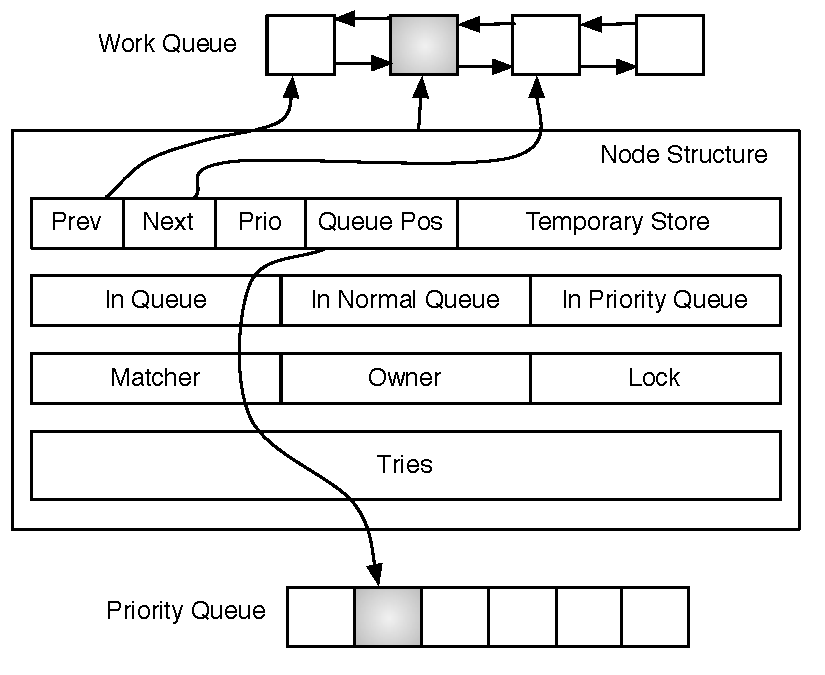
\includegraphics[width=0.5\textwidth]{node.pdf}}
    \caption{The node data structure.}
    \label{fig:node}
\end{figure}

The node data structure with an empty database occupies around 150 bytes.
In Fig.~\ref{fig:node} we present the node data structure and its fields. We summarize the data below:

\begin{description}
   \item[queue data]: Includes the field \texttt{Prev} (for the normal queue), \texttt{Next} (for the normal queue), \texttt{Prio} (priority) and \texttt{Queue Pos} (for the priority queue).
   \item[flags]: If the node is currently in the queue and in which queue. Includes \texttt{In Queue}, \texttt{In Normal Queue} and \texttt{In Priority Queue}.
   \item[temporary store]: A simple linked-list containing the unprocessed facts called \texttt{Temporary Store}.
   \item[database]: All the facts already processed which are true for this node. Is implemented as a trie and it is called \texttt{Tries}.
   \item[rule matcher]: The \texttt{Matcher} maintains the number of facts per predicate and which rules can be activated next. This is used for selecting the candidate rules.
   \item[owner]: Pointer to the owner thread. \texttt{Owner} in the figure.
   \item[lock]: A \texttt{Lock} mutex used to manipulate the node.
\end{description}
\end{comment}

\subsection{Work Stealing}

When a thread runs out of nodes to process, it will pick a thread at random and try to steal one node
from the target thread. The stealer thread will pop a node from either the priority queue or the normal queue. We use locks for mutual exclusion when dealing with those queues. Note that when a
node is stolen, its owner information also changes to the stealer thread.

It is important to note that whenever a node sends a coordination action fact to a node in another thread, the fact is ignored, due to the costs of sending
coordination data between threads. We intend to design an efficient mechanism to solve this problem.

In Fig.~\ref{code:work_loop} we present a simplified thread work loop that is executed in all threads. At each work cycle we check if thread has work in one of the two queues and if
not we attempt to steal a node from the other thread's queues. If our attempts to get some
work have succeeded, then we process the current node. Otherwise, the thread becomes idle and tries to synchronize and waits for the other threads to finish. Meanwhile, if the thread
receives some new node, \texttt{synchronize\_termination} will return \texttt{false} and
the thread will go to the next work cycle.

\begin{figure}[h!]
\small\begin{Verbatim}
void work_loop(thread_id tid) {
   while (true) {
      current_node = NULL;
      if(has_work(tid)) {
         current_node = pop_work(tid); // take node from one of the queues
      } else {
         // need to steal a node
         other = random_thread();
         current_node = steal_node_from_thread(other);
      }
      if(current_node == NULL) {
         become_idle(tid);
         if(synchronize_termination(tid))
            return;
         else
            become_active(tid);
      } else {
         process_node(current_node, tid);
      }
   }
}
\end{Verbatim}
  \caption{Thread work loop.}
  \label{code:work_loop}
\end{figure}

\section{Core Engine}\label{sec:core_engine}

Each node database is separated into two sets,
the database itself, and the \emph{temporary store}. The temporary store contains facts that have been
derived or have been sent to the node but have not been considered in rule derivations.
The temporary store exists for efficiency reasons because many linear facts are short-lived.

The temporary store is used to build the set of candidate rules that is represented as a priority queue.
To apply the rules, we take the highest priority rule from the queue and then run it.
If the derivation was successful, new facts may have been derived, thus we need to consider new
rules that are candidates from the newly derived facts and add them to the rule's priority queue.
On the other hand, when linear facts are consumed, some rules may not be applicable anymore and thus
we may need to remove them from the priority queue. In our implementation,
we keep a fact count for each predicate per node and also which predicates are needed for each rule. Whenever we have facts of some
predicates we can efficiently check if new rules are applicable for a specific node. We keep taking rules from the
queue until the queue is empty.

We do a small optimization to reduce the number of derivations of persistent facts. We
divide the program rules into two sets: \emph{persistent rules} and \emph{non persistent rules}.
Persistent rules are rules where only persistent facts are involved. We compile such rules
incrementally, that is, we attempt to fire all rules where a persistent fact is used. This is called
the \emph{pipelined semi-naive} evaluation and it originated in the P2 system~\cite{Loo-condie-garofalakis-p2}.
This evaluation method avoids excessing re-derivations of the same fact. The order of derivation does not matter for those rules, since
only persistent facts are used.

\section{Database}

The database is implemented using the trie data structure. Tries are trees where facts are indexed
by the common arguments. Because we need to delete facts from the database, we implement each trie level
as a double linked list so trie nodes can be easily removed. If a trie level has too many nodes, we
transform the linked list into a hash table in order to improve lookup.

Each node uses a trie per predicate to store facts. During matching of rules, we build a
\emph{match object}, which matches some arguments of the target predicate to instantiated values, so
that by searching the predicate trie from top to bottom, we can easily discard invalid trie branches.

\section{Summary}

This section provided a very brief overview of the current implementation of \lang. Although the parallel
and load balancing facilities of the runtime system are mostly completed, there is still some
implementation work to be done at the core engine level in order to make execution faster.
As it will be explained in Chapter~\ref{chapter:exp}, \lang is not yet competitive against
other systems, therefore we intend to perform more implementation work as part of this
thesis to make the virtual machine as fast as possible.

\chapter{Preliminary Experimental Results}\label{chapter:exp}
In this chapter we want to present some preliminary results of the \lang runtime system.
Firstly, we want to show that our virtual machine performs well when running multiple threads,
i.e., it can reasonably schedule the execution of programs to reduce execution time and increase parallel speedup. Secondly, we want to show that by using coordination directives, programs can perform faster.
Finally, we want to show that our programs are usually shorter than programs written in other languages.  

In our experimental setup, we used a machine with
four AMD Six-Core Opteron TM 8425 HE (2100 MHz) chips (24 cores) and 64 GB of DDR-2 667MHz (16x4GB) RAM,
     running GNU/Linux (kernel 2.6.31.5-127 64 bits).
     We compiled our virtual machine using GCC 4.4.5 (g++) with the flags \texttt{-O3 -std=c+0x -march=x86-64}.
     We run all experiments 3 times with the same configuration and then we averaged the run time.

\section{Parallel Experiments}

For the parallel results, we run each program using 1, 2, 4, 6, 8, 10, 12, 14 and 16 threads and compared the runtime against the execution of the sequential version of the virtual machine. We used the following programs:

\begin{description}
   \item[Greedy Graph Coloring (GGC)] in this program, we attempt to color each node of a graph so that no two adjacent nodes have the same color. We start with a small number of colors and then we expand the number of colors when we cannot color the graph.
   \item[PageRank] implements an asynchronous PageRank algorithm without synchronization between iterations. Every time a node sends a new rank to its neighbors and the change was significant, the neighbors are scheduled to recompute their ranks.
   \item[N queens] already explained before. We use an 11x11 board.
\end{description}

Figure~\ref{exp:graph_coloring} presents the speedup results for the GGC program using 3 different datasets. In the first plot, we show the speedup for a graph of 12,000 webpages. Since this dataset follows the power law, that is, there is a small number of pages with a lots of links (1\% of the nodes have 75\% of the edges), the speedup is not as good as the one shown when using a random dataset of 2,000 nodes, where each node has more or less the same number of links. In the weather graph 20\% of the nodes have 75\% of the edges, much less than the search engine dataset, and that shows in the results.

\newcommand{\figsize}[0]{6.5cm}

\begin{figure*}[htp]
   \centering
   \begin{subfigure}[b]{0.3\textwidth}
      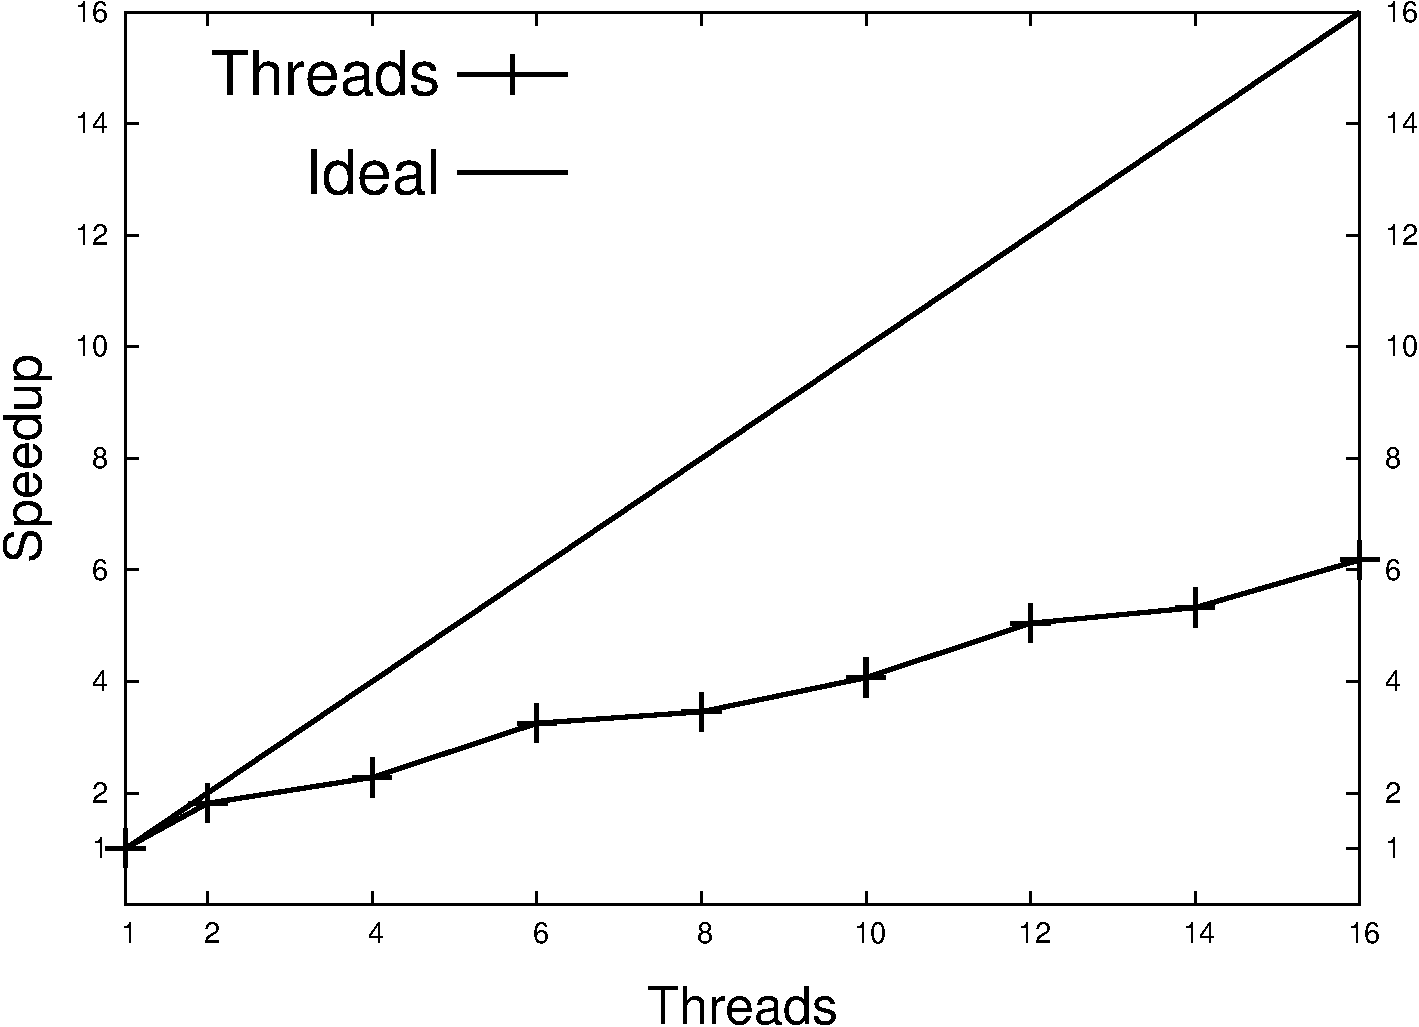
\includegraphics[width=\textwidth]{speedup_greedy-graph-coloring-search_engines.pdf}
      \caption{Search engine, a graph of web pages collected from a search engine (around 12,000 nodes).}
   \end{subfigure}
   \begin{subfigure}[b]{0.3\textwidth}
      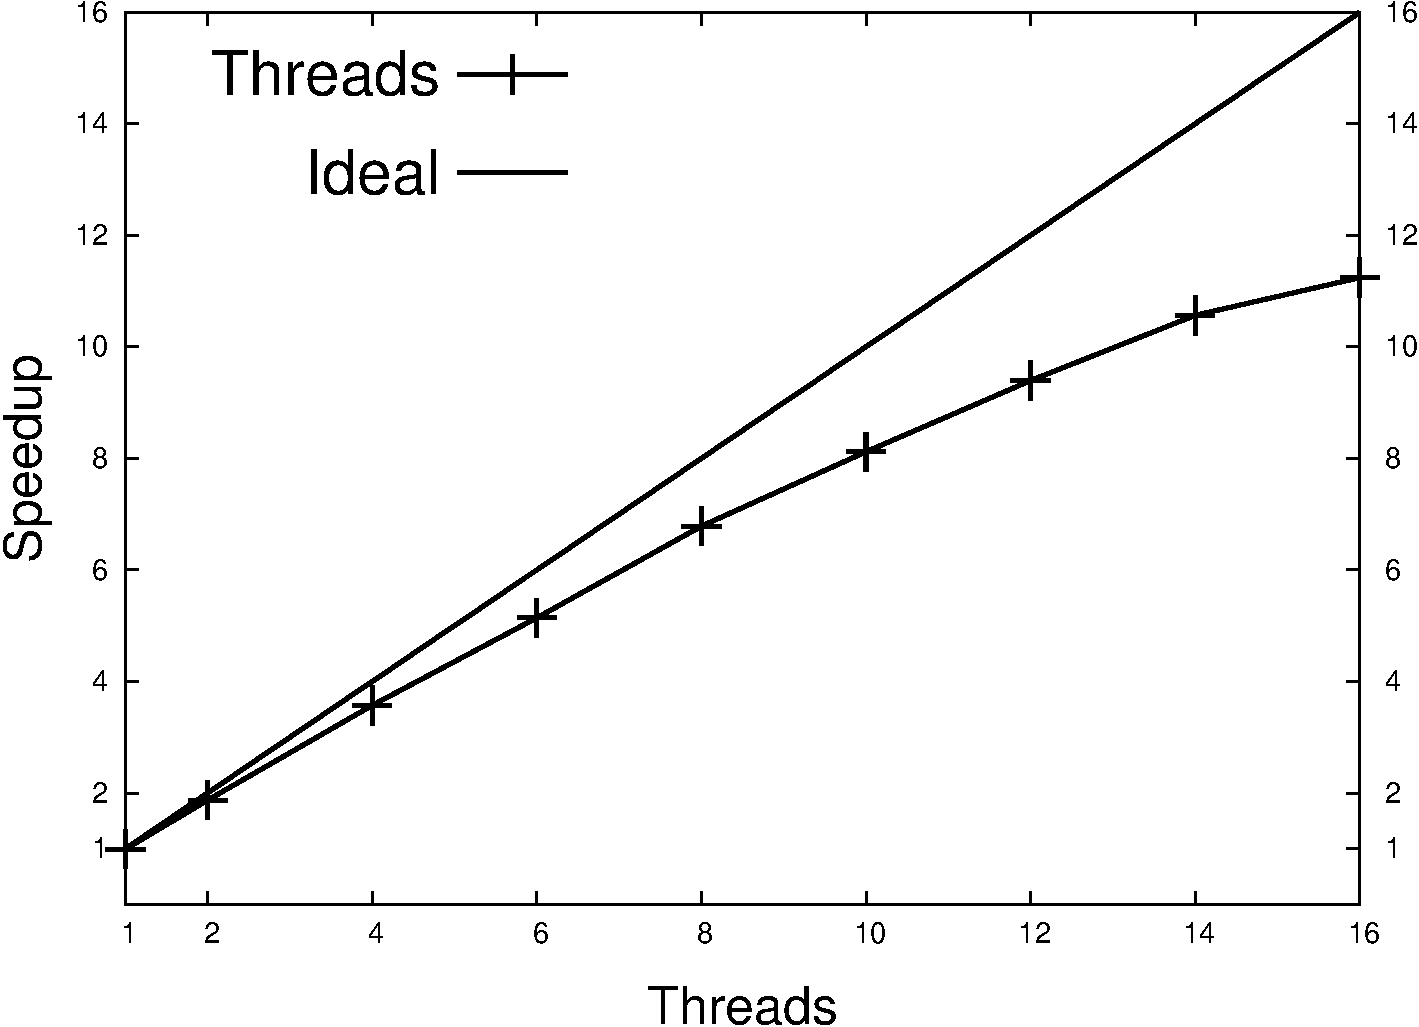
\includegraphics[width=\textwidth]{speedup_greedy-graph-coloring-weather.pdf}
      \caption{Weather, a graph of web pages collected from weather sites (around 8000 nodes).\newline}
   \end{subfigure}
   \begin{subfigure}[b]{0.3\textwidth}
      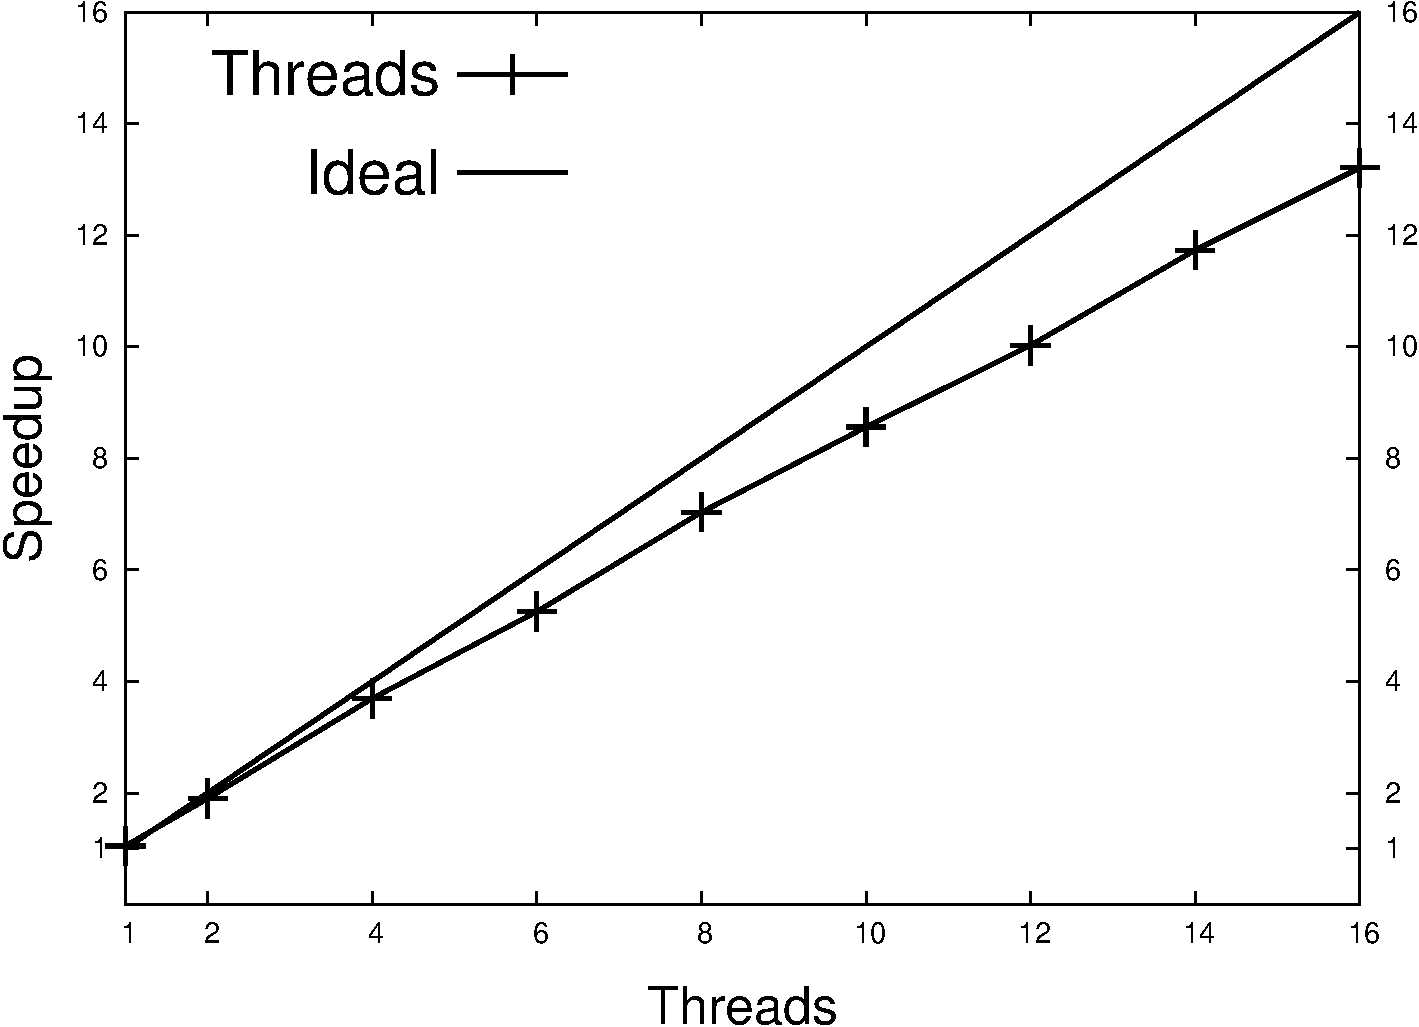
\includegraphics[width=\textwidth]{speedup_greedy-graph-coloring-2000.pdf}
      \caption{Using a random graph (with 2,000 nodes).\newline\newline}
   \end{subfigure}
   \caption{Experimental results for the greedy GGC algorithm.}
   \label{exp:graph_coloring}
\end{figure*}

\begin{figure*}[htp]
   \centering
   \begin{subfigure}[b]{0.3\textwidth}
      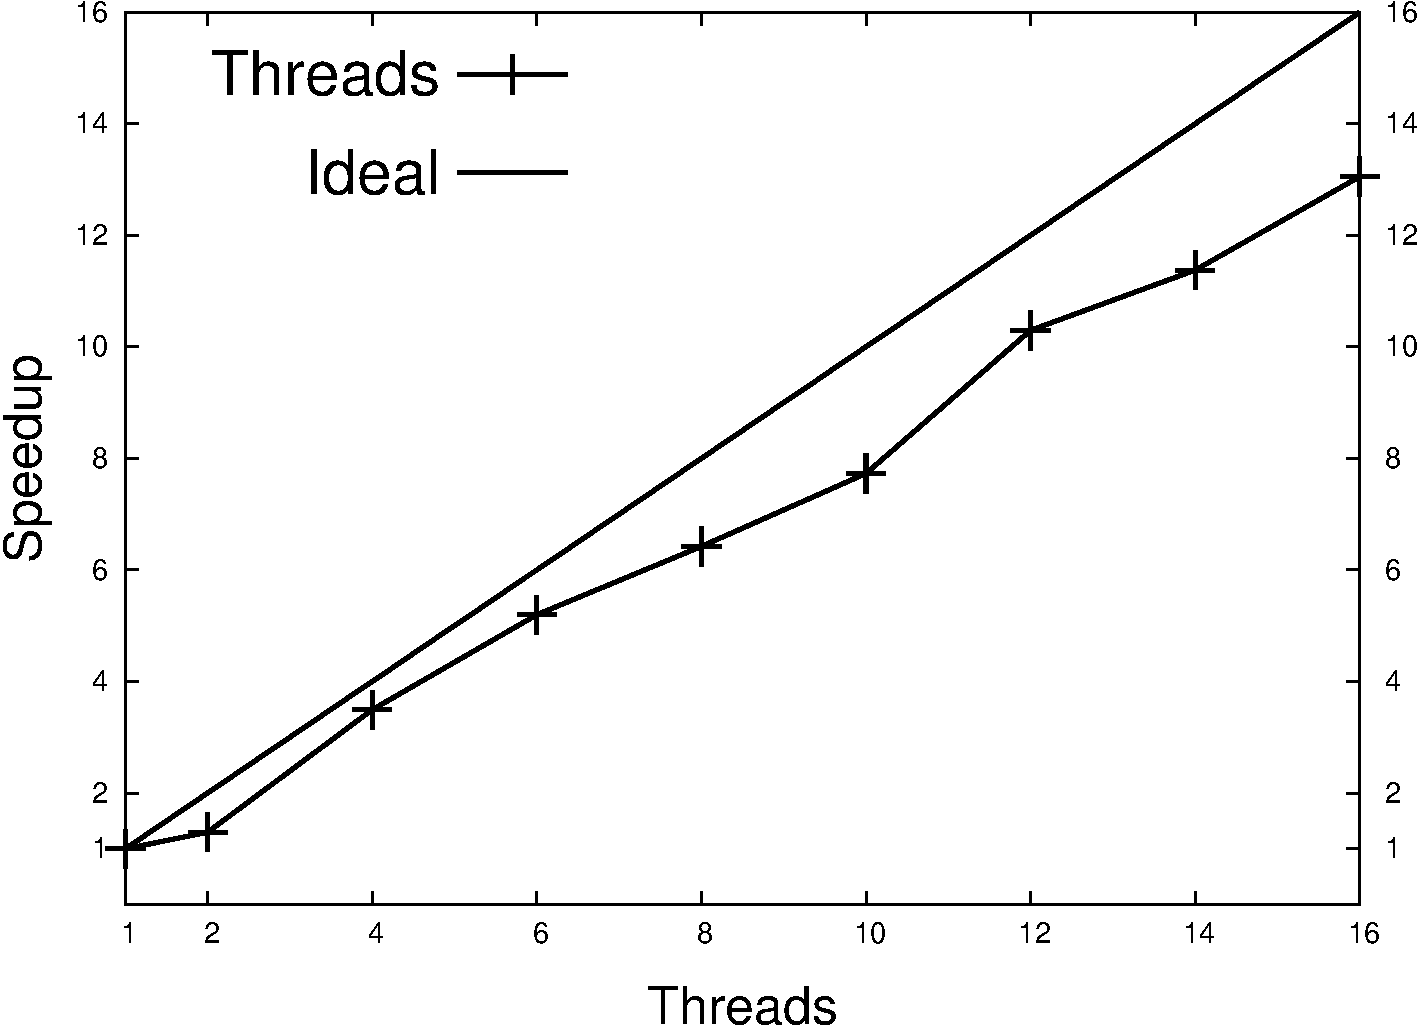
\includegraphics[width=\textwidth]{speedup_pagerank-search_engines.pdf}
      \caption{Search engine, a graph of web pages collected from a search engine (around 12,000 nodes)}
   \end{subfigure}
   \begin{subfigure}[b]{0.3\textwidth}
      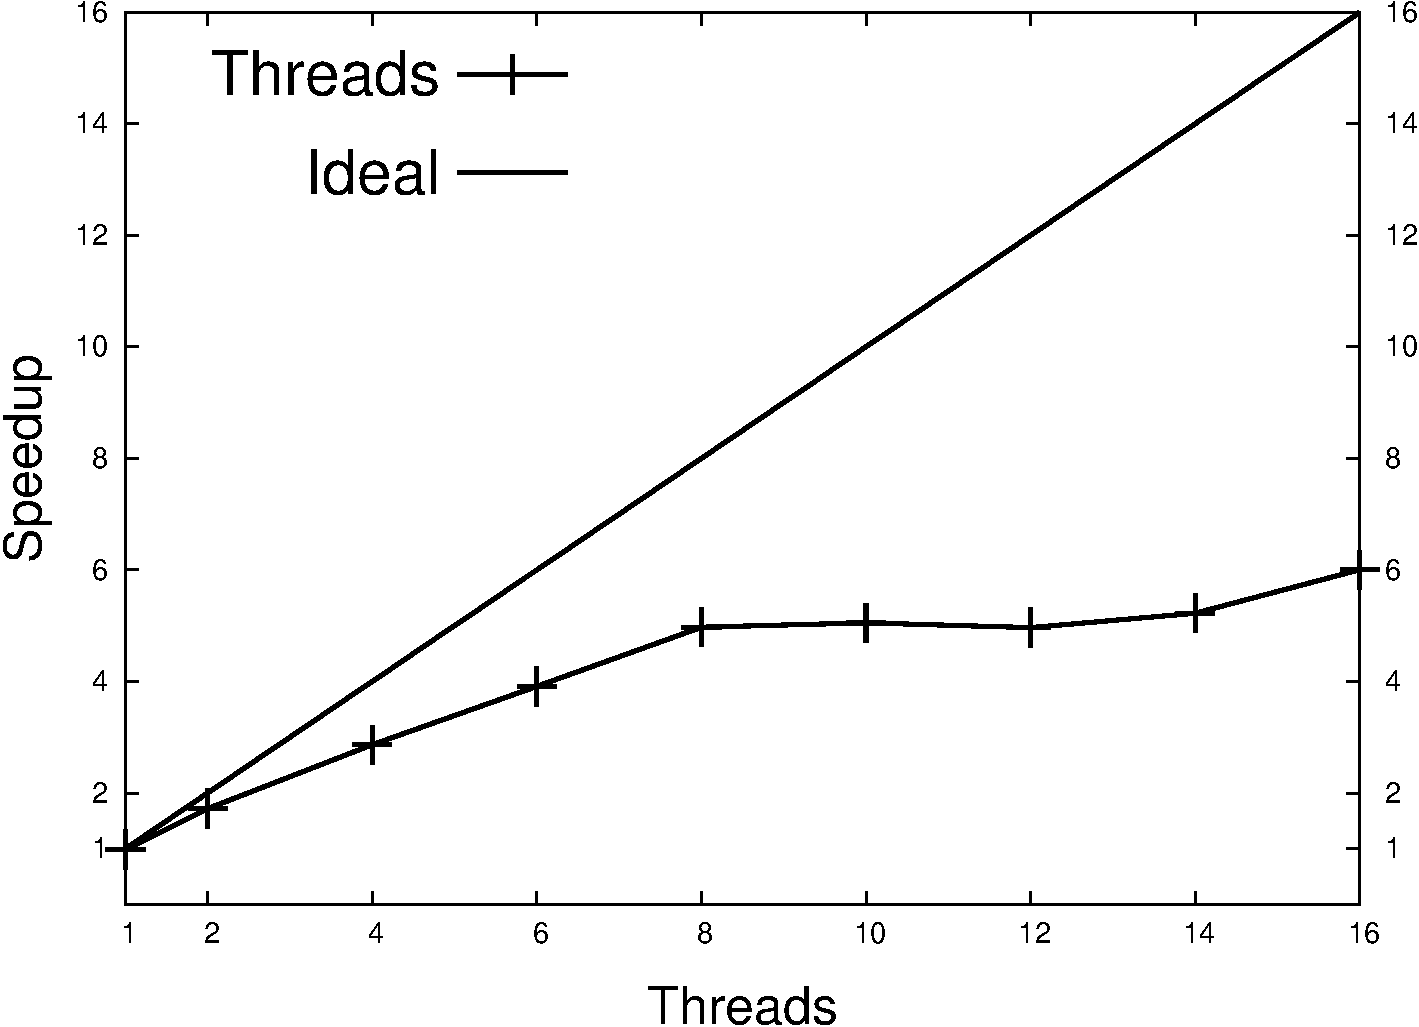
\includegraphics[width=\textwidth]{speedup_pagerank-movies.pdf}
      \caption{Movie, a graph of web pages collected from movie sites (around 8,000 nodes).\newline}
   \end{subfigure}
   \begin{subfigure}[b]{0.3\textwidth}
      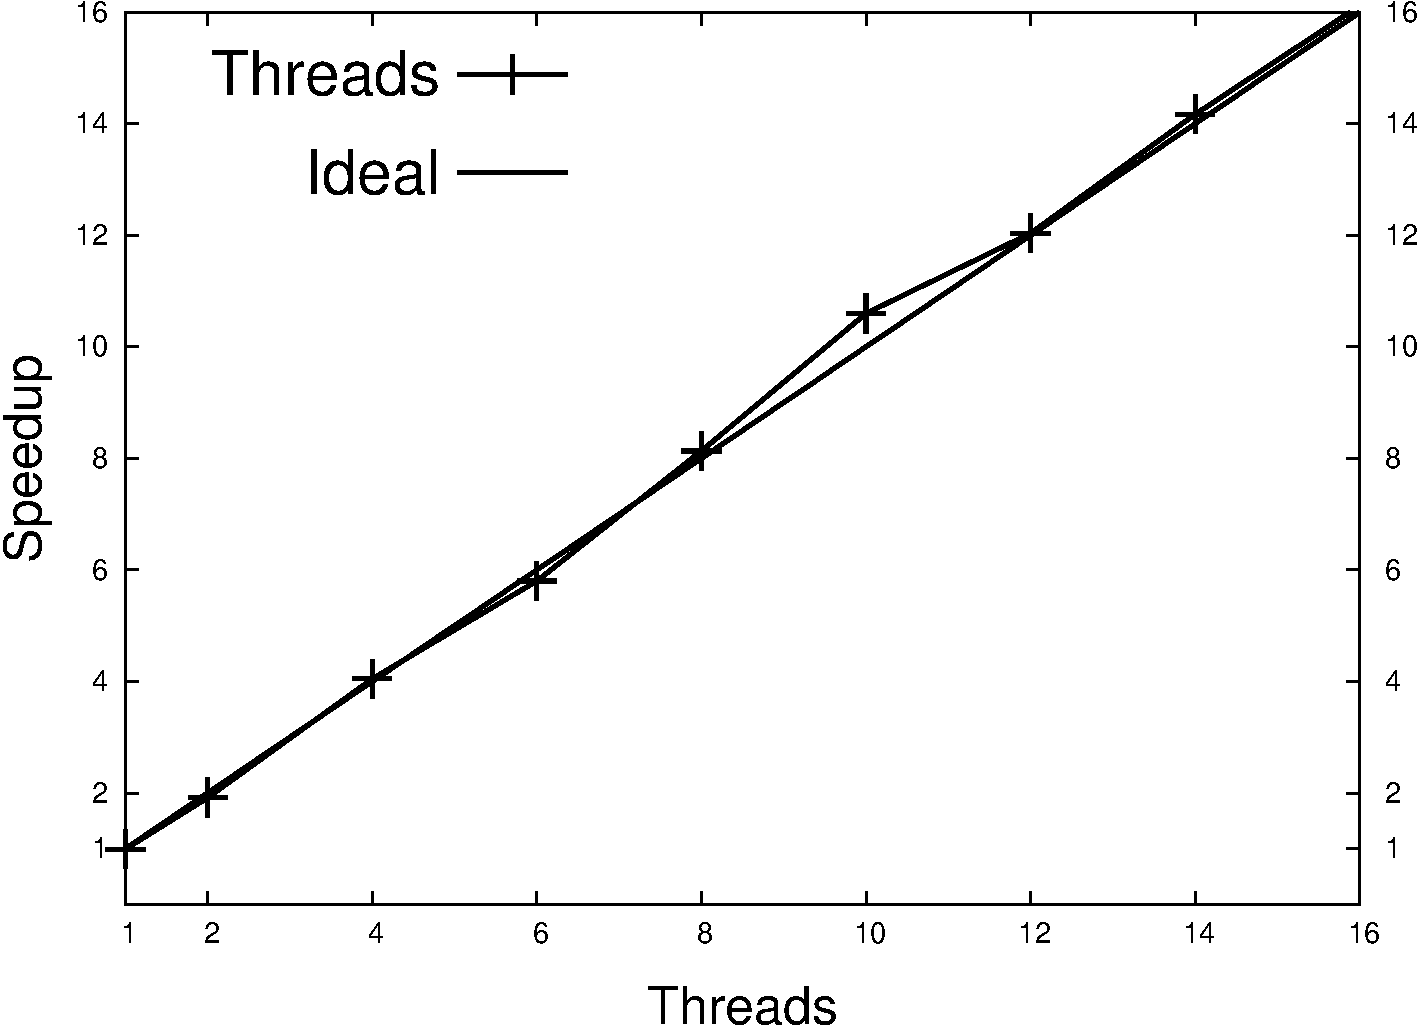
\includegraphics[width=\textwidth]{speedup_pagerank-500.pdf}
      \caption{Using a random, dense graph (with 500 nodes).\newline\newline}
   \end{subfigure}
   \caption{Experimental results for the asynchronous PageRank algorithm.}
   \label{exp:pagerank}
\end{figure*}

The PageRank results are shown in Fig.~\ref{exp:pagerank}. We have used the same search engine dataset as before and a new dataset representing movie websites \footnote{Both the search engine and movie graphs were retrieved from \url{http://www.cs.toronto.edu/~tsap/experiments/download/download.html}}. We notice that the search engine graph dataset is big enough to allow good execution improvements even with 16 threads, while the movie graph, being smaller, shows some scaling problems as the number of threads increases. Even though the search engine follows the power law it does not slowdown execution (as happened in the GGC program).
For the third plot, we used a random graph with 500 nodes and 75,000 edges. Since the graph is so dense, the runtime is capable of exploiting the
available parallelism, resulting in linear scalability.

\begin{figure}[h!]
     \centering
    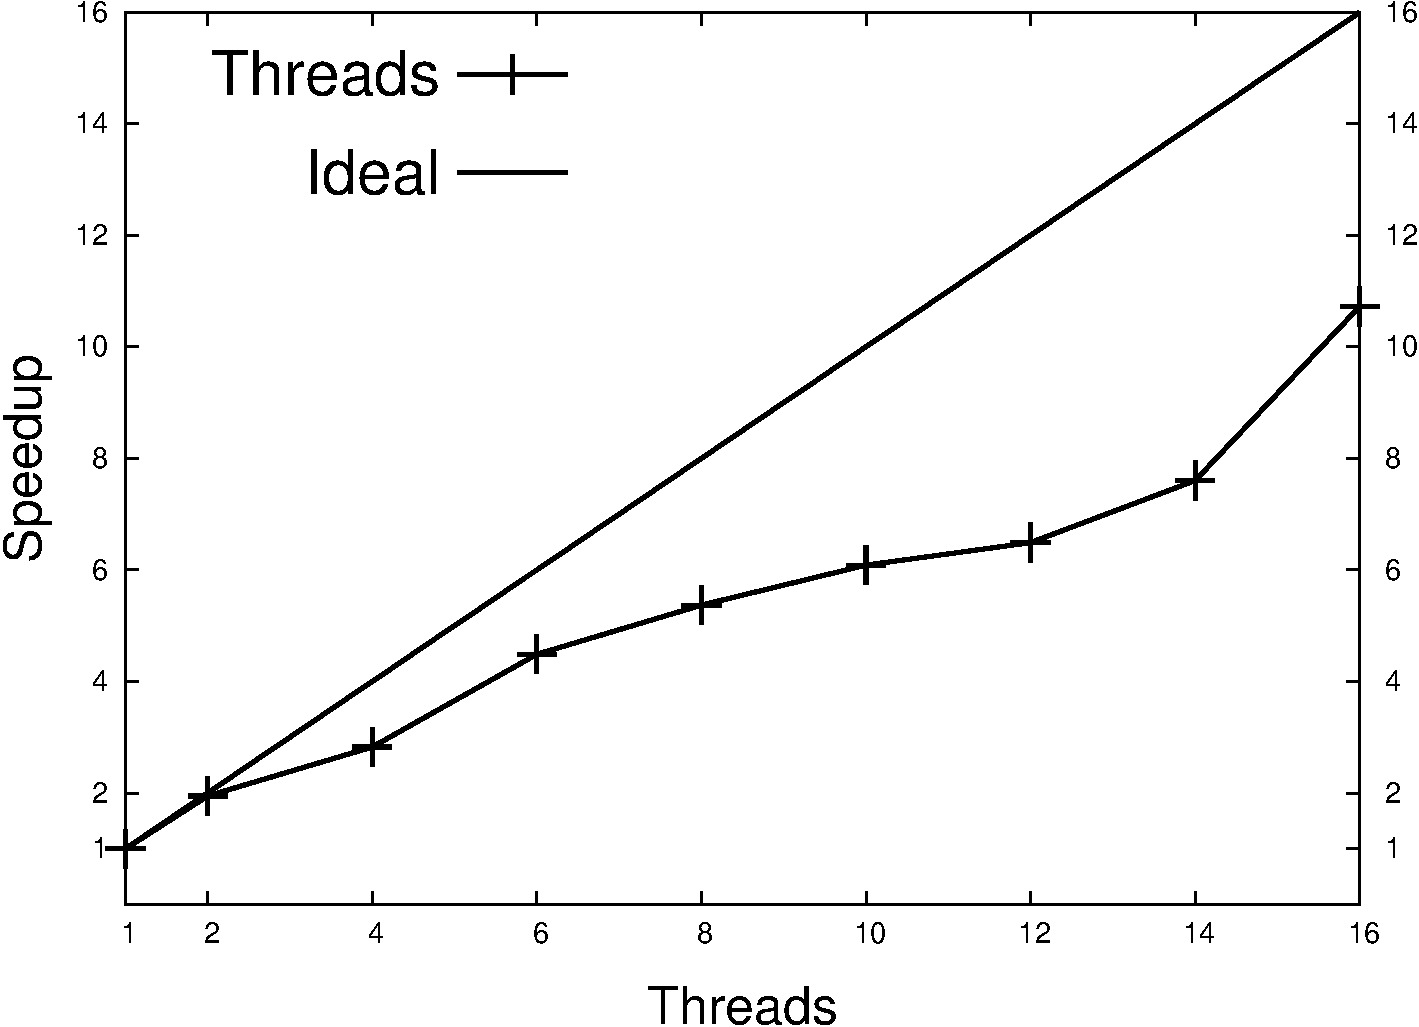
\includegraphics[width=0.4\textwidth]{speedup_8queens-11.pdf}
    \caption{Experimental results for the N queens program (11x11~board).}
    \label{exp:8queens}
\end{figure}

The results for the N queens program are shown in Fig.~\ref{exp:8queens}. This program is much less regular than the other two, since computation starts at the top of the grid and then rolls down, until only the last row is doing computation. Note that as the computation goes from row to row, the number of states increase, creating even more imbalances. The results show that our system is able to scale well with more traditional algorithms such as N Queens.

\section{Coordination Experiments}

In our coordination experiments, we are interested in showing that coordination improves the execution time of programs.
To do that, we used the following 3 programs:

\begin{description}
   \item[Heat Transfer] in the heat transfer program, we have a grid of cells that transfer heat with the neighbor cells by taking into account the edge weights. We use a dataset with a square of cells in the center of the grid with very high heat, while the outer cells have low heat. We use coordination to prioritize the neighbors of cells where rapid heat changes happen.
   \item[Single Source Shortest Path (SSSP)] we use the SSSP program shown earlier but we extended it to compute the distance to several nodes in order to increase the amount of computation.
   \item[Belief Propagation (BP)] this is the belief propagation program explained before. We build splash trees to improve performance.
\end{description}

Fig.~\ref{exp:heat-transfer} shows the results for the heat transfer program. \textbf{Threads} represents the speedup of the multicore execution
without coordination, while \textbf{Coord} represents the speedup when using coordination directives.
Both execution modes were compared against the sequential execution without coordination.
When using 1 thread, the coordinated version is almost 2 times
faster, however this speedup is slightly reduced as more threads are added. This happens because the \textbf{add-priority} action fact is ignored
when it is sent to a node located in a different thread.
Also note how the \textbf{Coord} line goes over the \textbf{Ideal} line, to the point where using 2 threads is 4 times faster than the sequential
version without priorities.

\begin{figure}[h!]
     \centering
   \begin{subfigure}[b]{0.4\textwidth}
      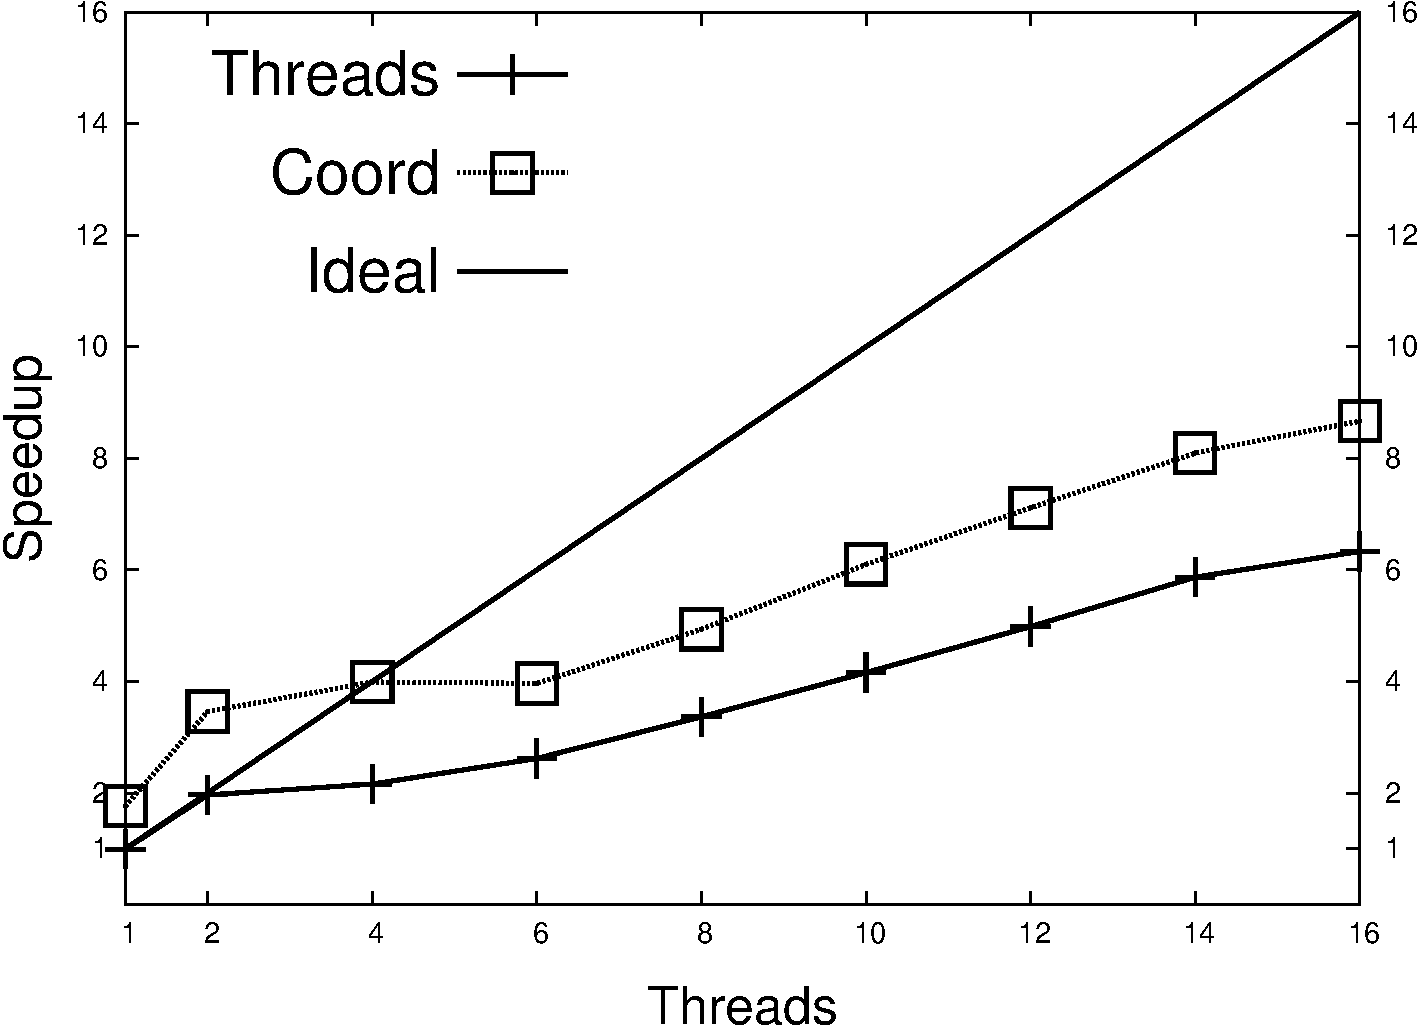
\includegraphics[width=\textwidth]{speedup_heat-transfer-80.pdf}
      \caption{HT program.\newline}\label{exp:heat-transfer}
   \end{subfigure}
   \begin{subfigure}[b]{0.4\textwidth}
      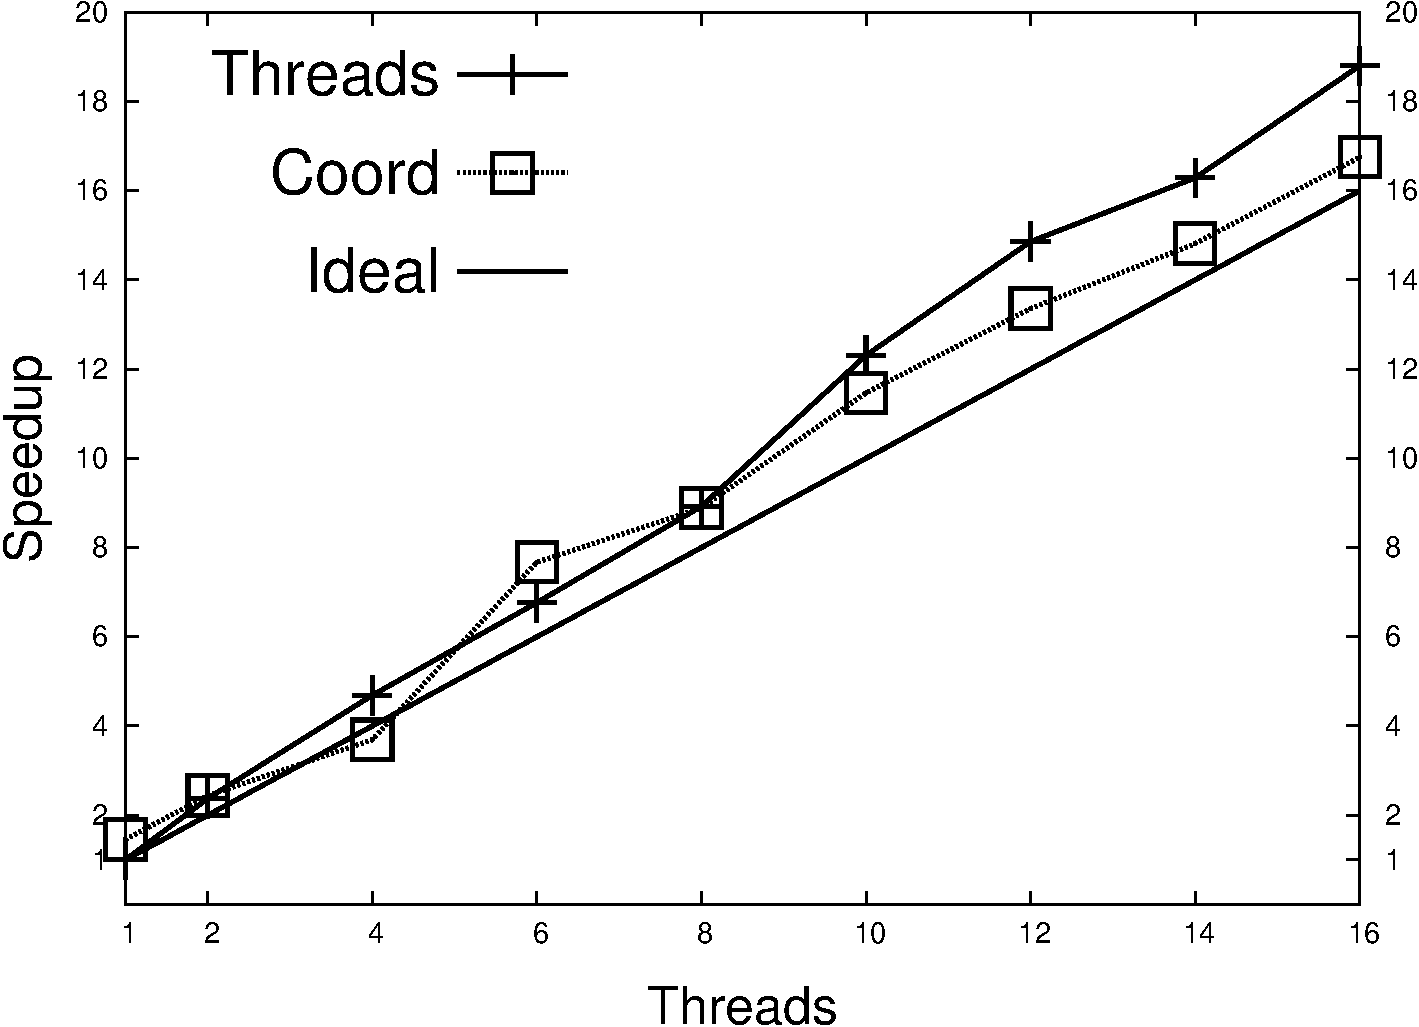
\includegraphics[width=\textwidth]{speedup_shortest-uspowergrid.pdf}
      \caption{SSSP program with the US Power Grid dataset.}\label{exp:sssp-uspowergrid}
   \end{subfigure}
   \caption{Experimental results for the HT and SSSP programs when using coordination.}
\end{figure}

To measure the performance of the SSSP program we used several datasets retrieved from \url{http://toreopsahl.com/datasets}. We computed several
statistics about each dataset, including: the number of nodes (\textbf{\# Nodes}), the number of edges (\textbf{\# Edges}) and
the average number of edges per node (\textbf{Edges / Node}). We also sorted the nodes by number of edges and counted the top number of nodes
with 25\% (\textbf{25\% Edges}), 50\% (\textbf{50\% Edges}) and 75\% (\textbf{75\% Edges}) of all edges.
These statistics and the speedup (\textbf{Speedup}) when using the coordinated version with 1 thread are presented in Table~\ref{tbl:shortest_path_speedup}.

We have tried to understand if there is a correlation between the graph structure and the coordination speedup. We can see that a higher number
of nodes and edges tends to improve execution. The US Airports dataset stands out because it is a small sized graph where a subset of airports
(70) have most connections. The other smaller datasets have a much stable distribution.
Still, the coordinated execution for most datasets is 30\% faster than the regular execution. We also included the speedup plot
for the US Power Grid dataset in Fig.~\ref{exp:sssp-uspowergrid} that compares the regular version against the coordinated version.
We note that the coordinated version loses its advantages as the number of threads increase. This may happen because we do not
use action facts that are sent between nodes in different threads.

\begin{table*}[ht]

\begin{center}
   \resizebox{16.5cm}{!}{
    \begin{tabular}{| l | c | c | c | c | c | c | c |}
    \hline
    \textbf{Dataset} & \textbf{Speedup} & \textbf{\# Nodes} & \textbf{\# Edges} & \textbf{Edges / Node} & \textbf{25\% Edges} & \textbf{50\% Edges} & \textbf{75\% Edges} \\ \hline \hline
    500 US Airports & 1.497 & 500 & 5960 & 11.92 & 14 & 37 & 70 \\ \hline
    US Power Grid & 1.459 & 4941 & 13188 & 2.67 & 485 & 1374 & 2131 \\ \hline
    Celegans Neural Network & 1.074 & 297 & 2345 & 7.89 & 24 & 65 & 104 \\ \hline
    Facebook like social network & 1.570 & 1899 & 20296 & 10.68 & 42 & 150 & 273 \\ \hline
    Intra-organizational network & 1.090 & 77 & 2288 & 28.94 & 9 & 24 & 36 \\ \hline
    \end{tabular}}
\end{center}
     \caption{Summarized information about the datasets used in the SSSP program.}
     \label{tbl:shortest_path_speedup}
\end{table*}

While the previous results were computed using only one thread, we also see good speedups with multiple threads. However, the gains reduce as we add
more threads because the decision of picking the best path is done at the thread level, thus reducing the opportunities for optimization.

For the BP program, we have a noisy image made of 400x400 pixels that needs to be denoised.
To put our implementation in perspective, we have also run the GraphLab (version 1) implementation of the same problem. The results are shown
in Fig.~\ref{exp:splashbp}. The first plot presents the scalability results for the simple BP problem. The GraphLab version
uses the \textbf{fifo} scheduler that works identically to the basic \lang scheduler.

\begin{figure*}[ht]
   \centering
   \begin{subfigure}[b]{0.3\textwidth}
      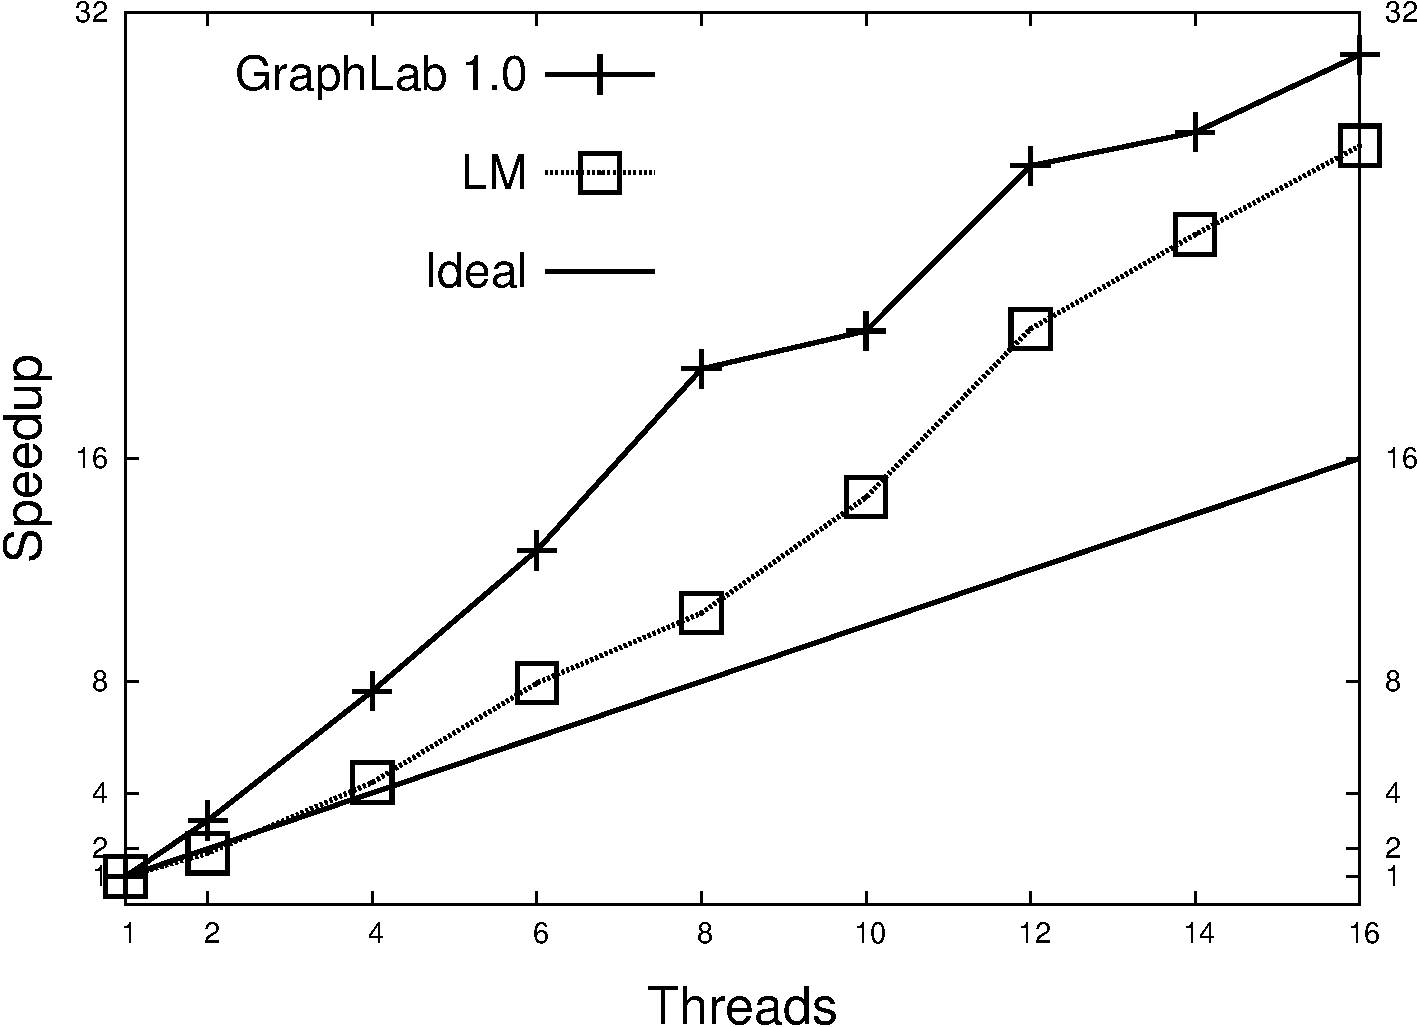
\includegraphics[width=\textwidth]{splash-bp-speedup1_csv.pdf}
      \caption{Scalability of basic BP.}
   \end{subfigure}
   \begin{subfigure}[b]{0.3\textwidth}
      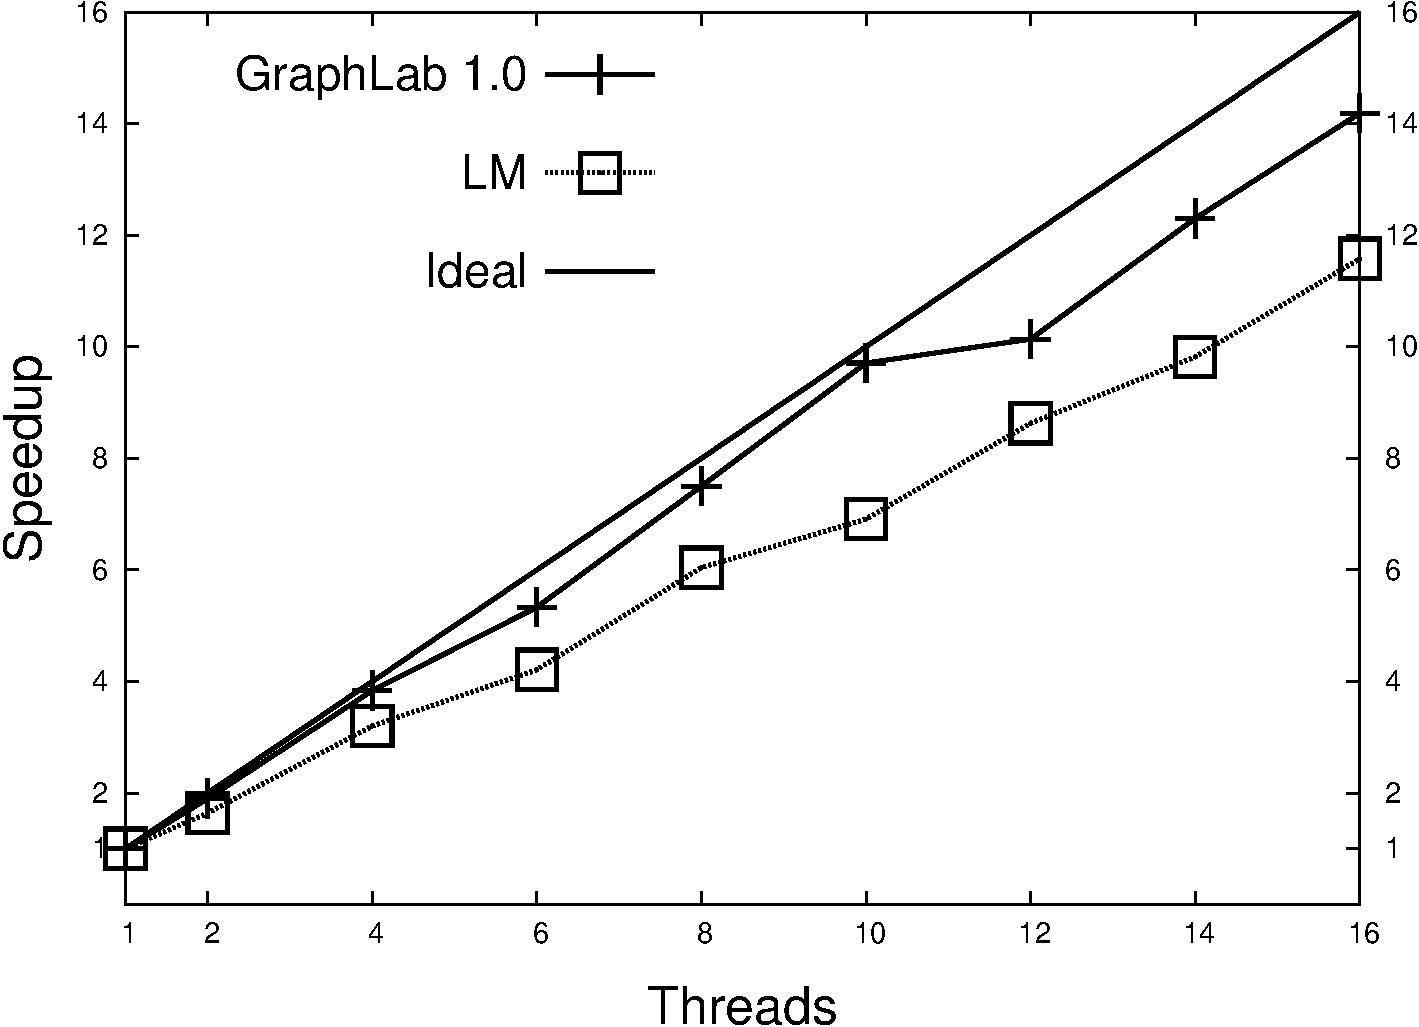
\includegraphics[width=\textwidth]{splash-bp-speedup2_csv.pdf}
      \caption{Scalability of BP with splashes.}
   \end{subfigure}
   \begin{subfigure}[b]{0.3\textwidth}
      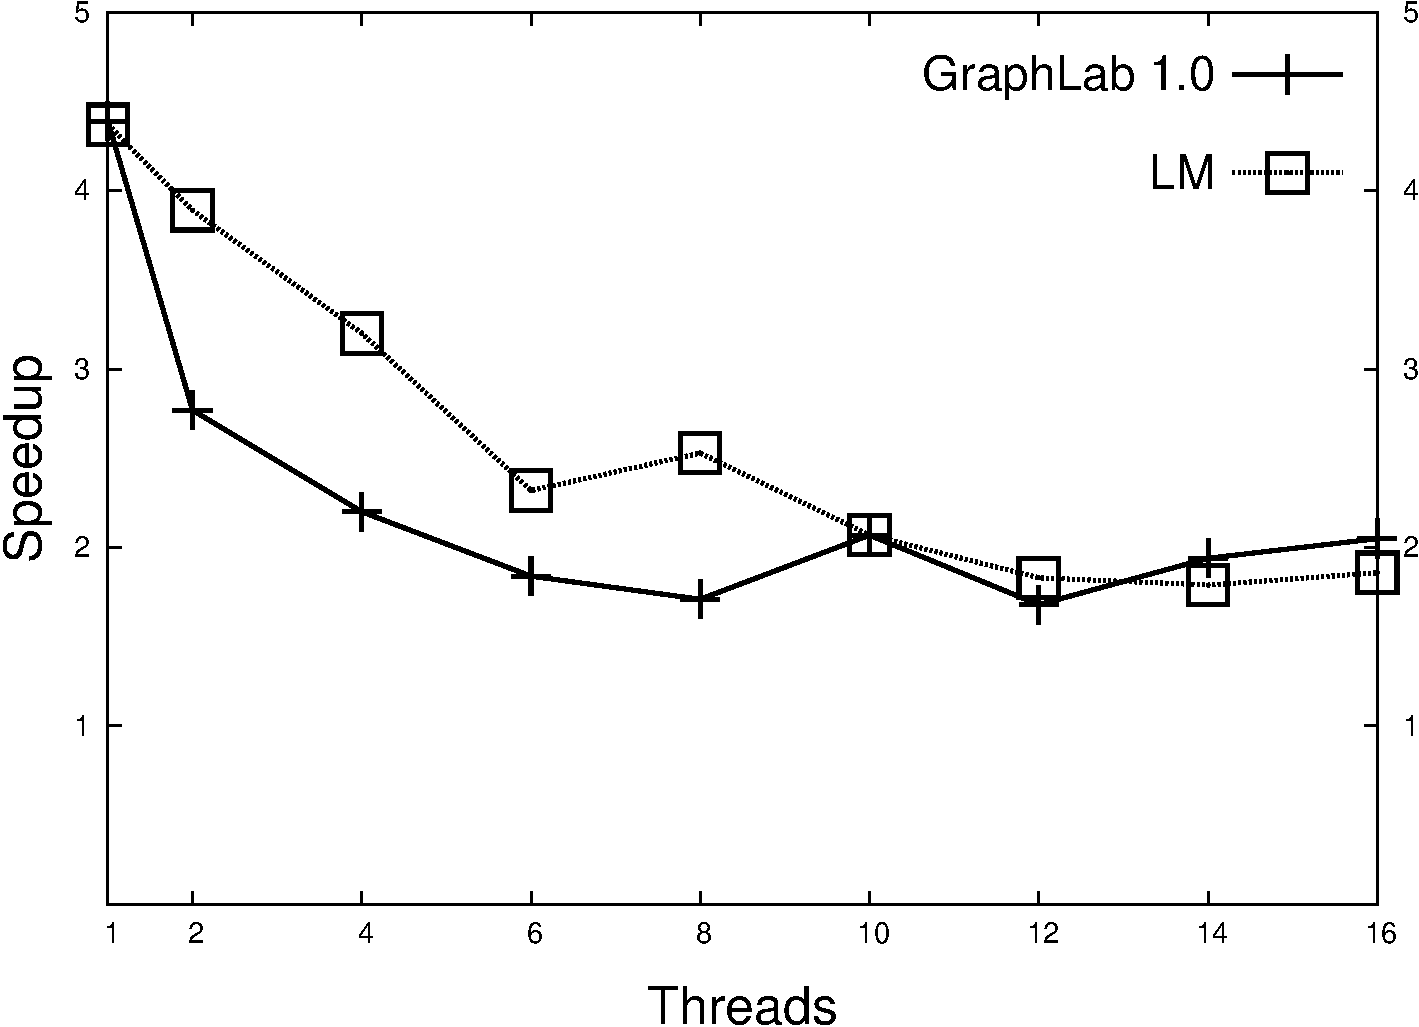
\includegraphics[width=\textwidth]{splash-bp-improv_csv.pdf}
      \caption{Coordination improvements by using splashes.}
   \end{subfigure}
   \caption{Experimental results for BP with coordination using splashes. The dataset is a 400x400 image.}
   \label{exp:splashbp}
\end{figure*}

The plot in Fig.~\ref{exp:splashbp}~(b) shows the scalability of the coordinated version. For GraphLab we used the \textbf{splash} scheduler, while \lang
runs with the extra coordination rules. Again, the scalability lines are very similar, but GraphLab appears to be slightly more scalable.
Finally, the last plot (Fig.~\ref{exp:splashbp}~(c)) presents the improvements of the coordinated version over the basic version when using a different
number of threads. With only 1 thread, we get almost a 5-fold speedup over the version without coordination. We can also see that adding more threads tends to reduce the effectiveness of splash trees in both systems.

In summary, using a small set of action facts and derivation rules we were able to implement complex
scheduling strategies similar to the ones present in GraphLab, a practical and powerful machine learning
framework.

\section{Language expressiveness and conciseness}

Finally, we show some results comparing the size of \lang programs against implementations of the same
programs in other languages. We want to show that \lang programs are more concise and can also be run in parallel from the start.

In table~\ref{tbl:length} we show how \lang programs compare against programs written in other languages in
terms of size. For the SSSP and the C version of N Queens~\cite{8queens-parallel} we are considering sequential implementations
that are very difficult to parallelize. Even so, \lang programs are much smaller and in our opinion, easier
to understand. For the N Queens problem, we also included an MPI implementation written in C~\cite{Rolfe:2008:SMA:1473195.1473217}
that is around 10 times longer than the \lang version. We are currently developing an MPI version
of the \lang runtime and preliminary results, also show some good speedups for this program.

\begin{table}[ht]
\begin{center}
   \resizebox{12cm}{!}{
    \begin{tabular}{| c | c | l | c |}
    \hline
    \textbf{Program} & \textbf{\lang} & \textbf{Others} & \textbf{Average} \\ \hline \hline
    SSSP & 6 & 25 (C++) & 24\% \\ \hline
    PageRank & 30 & 60 (GraphLab) & 50\% \\ \hline
    BP & 50 & 90 (GraphLab) & 55\% \\ \hline
    Splash BP & 50 & 350 (GraphLab) & 14\% \\ \hline
    N Queens & 40 & 300 (C~\cite{8queens-parallel}), 400 (MPI~\cite{Rolfe:2008:SMA:1473195.1473217}) & 11\% \\ \hline
    \end{tabular}}
\end{center}
     \caption{Comparison of source code size against other languages.}
     \label{tbl:length}
\end{table}

The GraphLab versions of PageRank, BP and Splash BP are all written in C++ and can be run in
parallel. We only counted the bare minimum number of lines for these programs (the update function)
so that our analysis is not biased towards \lang. The \lang versions of PageRank and BP are around
half of the size of the GraphLab versions. However, \lang really shines in the Splash BP program because
the code is much more concise than the corresponding code of GraphLab.

\section{Comparison Against Other Systems}

We also made some absolute runtime comparisons of \lang programs with the same programs written in
other languages such as Prolog, Python and C/C++.

In our experiments, the N Queens program runs
more than 100 times slower when compared to a C implementation and 30 times slower than a Python
implementation. The PageRank algorithm runs around 20 times slower than the identical GraphLab
implementation and the SSSP program runs 60 times slower than the C version.

Previously, we have seen that the \lang version of Splash BP program has the same scalability pattern
as GraphLab (Fig.~\ref{exp:splashbp}), however our experiments show that \lang runs about 3 to 4 times slower in absolute terms. This is better than the other comparisons and can be explained by the fact
that most computation is done inside external C functions and not applying rules.

We can see a correlation between the number of rules applied and facts derived and execution time.
Because our virtual machine is still a work in progress, we can see plenty of optimization opportunities
to improve these results.

\section{Summary}

This section gave some evidence to our thesis that \lang programs are concise and scalable. Moreover, we
also showed that coordination directives have potential to improve the execution time
of programs. Our coordination code is also far shorter than competing systems such as GraphLab, which is
very promising. However, the \lang runtime system is still not competitive in some areas, specially
when deriving and consuming a huge number of facts.

\chapter{Road Map}

In this chapter we propose a research roadmap that will allows to fully establish the validity of our thesis.
Our experimental results have shown promising results, although this still some work to be done to make
\lang more usable in real world applications.

\section{Compilation and Runtime Improvements}

As we have seen in Chapter~\ref{chapter:exp}, \lang is able to scale programs reasonably well
in multicore architectures.
The use of coordination directives also help us improve the execution time of programs. However,
when we compare the absolute execution time of programs against comparable implementations in
languages such as C or Prolog, \lang is still not very competitive since it is many times slower.

Although compiled \lang programs are byte-code interpreted, which is a natural
source of overhead, we think this is still the best architecture for our system and the overhead
is on the naïve compilation of programs. \lang programs can take advantage of the fact that
\lang is logic-based language and thus it is possible to optimize and simplify the execution of rules
if we prove that facts follow certain properties and constraints.

We think that a big chunk of execution time is spent doing
database operations such as matching and fetching sets of candidate facts.
However, some programs such as N Queens are very computationally expensive since they have
a lot of list manipulation operations.

\subsection{Overhead Analysis}

To better understand the sources of overhead of our virtual machine, we propose doing a series
of experiments to understand where the most execution time is spent. We will gather the following
items:

\begin{itemize}
   \item \textbf{Database search operations}
   
   Measure the time spent fetching or searching facts from the database.
   
   \item \textbf{Database insertion operations}
   
   Measure the time spent inserting facts into the database.
   
   \item \textbf{Database removal operations}
   
   Measure the time spent removing facts from the trie.
   
   \item \textbf{Temporary store operations}
   
   Measure the time looking for facts in the temporary store.
   
   \item \textbf{Rule engine}
   
   Measure the time spent calculating which rules must be scheduled to run and the time for managing the priority queue of rules.
   
   \item \textbf{Rule measurement}
   
   Measure the time spent executing each rule of the program.
   
   \item \textbf{Fact statistics}
   
   Measure the number of facts derived and consumed for each predicate.
   
   \item \textbf{Communication overhead}
   
   Measure the communication overhead between threads.
   
\end{itemize}

\subsection{Preliminary Optimization Ideas}

After doing the previous analysis for each \lang program, we intend to try different VM optimizations, namely.

\begin{itemize}
   \item \textbf{Improve database indexing}
   
   Sometimes we need to search for facts where the second argument is a constant. It would be better to put the second argument at the top of trie in order to prune the most branches as soon as possible. We intend to employ a smarter compilation strategy, where we re-order the body of a rule to increase the number of such constraints and give information to the runtime system of the optimal ordering the the trie.
   
   \item \textbf{Improve temporary store}
   
   Currently the temporary store is just a simple linked list. We also need to look into the temporary store when rules are executed. If the temporary store is heavily used (which we think it is) we want to use an improve data structure.
   
   \item \textbf{Experiment other data structures for the database}
   
   Although the trie is good general data structure, it may not be optimal for certain types of predicates. For example, if a predicate has only one argument it may be best to just use a simple array, where each array position is the value of the argument. We should improve the runtime if the number of such facts is small.
   
   \item \textbf{Reduce communication overhead between nodes}
   
   When a thread needs to send a fact to another node that is located on that same thread, there is a certain overhead because we assume that other threads will also perform the same operation. We want to improve this by using specialized operations for nodes in the same thread. However, we need to pay attention to the use of work stealing since nodes sometimes are moved between threads.
   
   \item \textbf{Improve removal of facts from the database}

   If a fact needs to be removed from the database, we simply remove the corresponding branch from the trie. However, if the same fact is derived later on and asserted into the database, it is potentially better to not remove the trie nodes but keep them for later use.
   
   \item \textbf{JIT compilation of computation heavy rules}
   
   If some rules use a lot of mathematical or list operations it may be worth trying to compile them into machine code instead of using interpreted byte-code.
\end{itemize}

\subsection{Invariant Optimizations}

While the previous optimizations will probably yield some good improvements, we think that the biggest
improvements can be reached by using invariant optimizations. By this, we mean proving certain
properties about the program and its facts and then compiling the program accordingly.

\begin{itemize}
   
   \item \textbf{Property facts}
   
   In most programs there is a set of linear facts that act as a field of the node. These facts may
   be consumed and derived but they are never consumed because only their arguments change.
   For example:

\begin{Verbatim}
a(A, X), b(A, X) -o a(A, Y).
\end{Verbatim}

   In this case we consume \texttt{a(A, X)} but we derive another \texttt{a(A, Y)} with a different
   second argument. We want to prove that, for certain predicates, at any point in time there is only one
   set of facts of that predicate and although they may be consumed, only the arguments change.
   With this analysis, we can improve the code to avoid unnecessary re-derivations.
   
   \item \textbf{Triggering linear facts}
   
   Some facts never really trigger the execution of rule, because most rules need one or two special facts that
   will activate the rule. Those facts are derived in only a few rules and are intermittently consumed and
   re-derived. All the non-triggering facts never activate the execution of rules because they may be
   property facts and are constantly present in the database.
   We must prove which predicates potentially trigger the execution of rules and mark them as such.
   
   \item \textbf{Single use facts}
   
   Single use facts are a special case of triggering linear facts because once they are derived they are
   proven to be immediately consumed. The following example shows the only place in the program where
   the \texttt{a} predicate is used in the body of the rule. Note that no matter what the state of
   the database is, we can prove that \texttt{a} facts can be used immediately and will work as a function
   call in imperative languages.
   
   \begin{Verbatim}
   .... -o a(A, 2).

a(A, 1) -o ....
a(A, 2) -o ....
a(A, 3) -o ....

   ....
   \end{Verbatim}
    
\end{itemize}

Note that these are only preliminary invariant optimizations. More optimization ideas will appear
as we look further into our programs and find general patterns.

\subsection{Measurements}

After implementing all the needed optimizations, we want to measure the effect of each optimization
and relate each program to the optimizations used.

Finally we want to systematically compare \lang execution against execution of the identical programs
in languages such as C, Python, Haskell and Prolog. While we do not expected to run as fast as C,
we expect \lang programs to be competitive against Python, Haskell or Prolog.

\section{Coordination \& Programs}

We want to implement more programs that use coordination. By implementing new programs we can
extend the set of coordination directives and find out which action or sensing facts may be
appropriate in our system. We are specially interested in designing more sensing and action
facts that place nodes in specific threads to improve data locality.

A potential algorithm that we can implement is the Alpha-Beta search algorithm. It is a good program
because we can reduce the search space by prioritizing certain tree branches. It remains to be
seen if the program can be easily implemented in \lang.
We intend to measure the execution speedup of these new coordinated programs.

In terms of implementation, our virtual machine ignores action facts for coordination when a fact
is exchanged between nodes of different threads. We want to design new mechanisms
that will efficiently handle such situations so that action facts are taken into account without
slowing down execution due to thread synchronization.

\section{Planned Schedule}

The proposed work is scheduled on a 18 month timeline ending May 2015.

\begin{itemize}
   \item \textbf{Spring 2014}
      
   Perform the overhead analysis for the current set of \lang programs.
   Spend some time improving upon the preliminary optimization ideas and implement them.

   Prove the cut-elimination theorem of our linear logic fragment. Baelde's work~\cite{Baelde:2012:LGF:2071368.2071370} will make this easy.
   
   \textbf{Checkpoint}: new benchmarks for \lang programs taking into account the new optimizations.

   \item \textbf{Summer 2014}
   
   Design a set of invariant optimizations and implement them in the compiler. Meanwhile, benchmark the runtime of programs to see how they improve the execution.

   Writing a few more programs using coordination.
   Meanwhile extend the set of coordination directives that will help implement the new programs.

   \textbf{Checkpoint}: new benchmarks for \lang programs and their comparison against other implementations.
   
   \item \textbf{Fall 2014}
   
   Continue working on invariant optimizations.
   Build website for \lang and the make \lang system publicly available.
   
   \textbf{Checkpoint}: The \lang website. Improved benchmark results for \lang programs.
   
   \item \textbf{Spring 2015}
   
   Write the thesis document.
   
   \textbf{Checkpoint}: thesis defense.

\end{itemize}

\appendix
%\chapter{Low Level Dynamic Semantics}\label{low_level_semantics}

\footnotesize

\subsubsection{Application}

\[
\infer[\ao start \; matching]
{\ao \Gamma; \Delta; A \lolli B; R \rightarrow \Xi'; \Delta'; \Gamma'}
{\mo \Gamma; \Delta; \cdot; \cdot; A; B; \cdot; R \rightarrow \Xi'; \Delta'; \Gamma'}
\]

\[
\infer[\doo rule]
{\doo \Gamma; \Delta; R, \Phi \rightarrow \Xi'; \Delta';\Gamma'}
{\ao \Gamma; \Delta; R; (\Phi, \Delta) \rightarrow \Xi';\Delta';\Gamma'}
\]


\subsubsection{Match}

\[
\infer[\mo p \; ok \; first]
{\mo \Gamma ; \Delta, p_1, \Delta'' ; \Xi; p, \Omega; H; \cdot; R \rightarrow \Xi'; \Delta'; \Gamma'}
{\mo \Gamma ; \Delta, \Delta''; \Xi, p_1; \Omega; H; (\Delta, p_1; \Delta''; p; \Omega; \Xi; \cdot; \cdot); R \rightarrow \Xi'; \Delta'; \Gamma'}
\]

\[
\infer[\mo p \; ok \; other \; q]
{\mo \Gamma ; \Delta, p_1, \Delta'' ; \Xi; p, \Omega; H; C_1, C; R \rightarrow \Xi'; \Delta'; \Gamma'}
{\begin{split}\mo &\Gamma ; \Delta, \Delta''; \Xi, p_1; \Omega; H; (\Delta, p_1; \Delta''; p; \Omega; \Xi; q, \Lambda; \Upsilon), C_1, C; R \rightarrow \Xi'; \Delta'; \Gamma' \\ C_1 &= (\Delta_{old}; \Delta'_{old}; q; \Omega_{old}; \Xi_{old}; \Lambda; \Upsilon)\end{split}}
\]


\[
\infer[\mo p \; ok \; other \; \bang q]
{\mo \Gamma ; \Delta, p_1, \Delta'' ; \Xi; p, \Omega; H; C_1, C; R \rightarrow \Xi'; \Delta'; \Gamma'}
{\begin{split}\mo &\Gamma ; \Delta, \Delta''; \Xi, p_1; \Omega; H; (\Delta, p_1; \Delta''; p; \Omega; \Xi; \Lambda; q, \Upsilon), C_1, C; R \rightarrow \Xi'; \Delta'; \Gamma' \\ C_1 &= [\Gamma_{old}; \Delta_{old}; \bang q; \Omega_{old}; \Xi_{old}; \Lambda; \Upsilon]\end{split}}
\]

\[
\infer[\mo p \; fail]
{\mo \Gamma ; \Delta; \Xi; p, \Omega; H; C; R \rightarrow \Xi'; \Delta'; \Gamma'}
{p \notin \Delta & \cont C ; H; R; \Gamma; \Xi'; \Delta'; \Gamma'}
\]

\[
\infer[\mo \bang p \; ok \; first]
{\mo \Gamma, p, \Gamma'' ; \Delta; \Xi; \bang p, \Omega; H; \cdot; R \rightarrow \Xi'; \Delta'; \Gamma'}
{\mo \Gamma, p, \Gamma'' ; \Delta; \Xi; \Omega; H; [\Gamma''; \Delta; \bang p ; \Omega; \Xi; \cdot; \cdot]; R \rightarrow \Xi'; \Delta'; \Gamma'}
\]

\[
\infer[\mo \bang p \; ok \; other \; q]
{\mo \Gamma, p, \Gamma'' ; \Delta; \Xi; \bang p, \Omega; H; C_1, C; R \rightarrow \Xi'; \Delta'; \Gamma'}
{\begin{split}\mo &\Gamma, p, \Gamma'' ; \Delta; \Xi; \Omega; H; [\Gamma''; \Delta; \bang p ; \Omega; \Xi; q, \Lambda; \Upsilon], C_1, C; R \rightarrow \Xi'; \Delta'; \Gamma' \\ C_1 &= (\Delta_{old}; \Delta'_{old}; q; \Omega_{old}; \Xi_{old}; \Lambda; \Upsilon)\end{split}}
\]


\[
\infer[\mo \bang p \; ok \; other \; \bang q]
{\mo \Gamma, p, \Gamma'' ; \Delta; \Xi; \bang p, \Omega; H; C_1, C; R \rightarrow \Xi'; \Delta'; \Gamma'}
{\begin{split}\mo &\Gamma, p, \Gamma'' ; \Delta; \Xi; \Omega; H; [\Gamma''; \Delta; \bang p ; \Omega; \Xi; \Lambda; q, \Upsilon], C_1, C; R \rightarrow \Xi'; \Delta'; \Gamma' \\ C_1 &= [\Gamma_{old}; \Delta_{old}; \bang q; \Omega_{old}; \Xi_{old}; \Lambda; \Upsilon]\end{split}}
\]

\[
\infer[\mo \bang p \; fail]
{\mo \Gamma ; \Delta; \Xi; \bang p, \Omega; H; C; R \rightarrow \Xi'; \Delta'; \Gamma'}
{p \notin \Gamma & \cont C; H; R; \Gamma; \Xi'; \Delta'; \Gamma'}
\]

\[
\infer[\mo \otimes]
{\mo \Gamma ; \Delta; \Xi; A \otimes B, \Omega ; H ; C; R \rightarrow \Xi'; \Delta';\Gamma'}
{\mo \Gamma ; \Delta; \Xi; A, B, \Omega; H; C; R \rightarrow \Xi';\Delta';\Gamma'}
\]

\[
\infer[\mo end]
{\mo \Gamma ; \Delta; \Xi; \cdot ; H; C; R \rightarrow \Xi'; \Delta'; \Gamma'}
{\done \Gamma ; \Delta; \Xi; \cdot ; H; \cdot \rightarrow \Xi'; \Delta'; \Gamma'}
\]

\subsubsection{Continuation}

\[
\infer[\cont next \; rule]
{\cont \cdot; H; (\Phi, \Delta); \Gamma ; \Xi'; \Delta'; \Gamma'}
{\doo \Gamma; \Delta; \Phi \rightarrow \Xi'; \Delta'; \Gamma'}
\]

\[
\infer[\cont p \; next]
{\cont (\Delta; p_1, \Delta''; p, \Omega; \Xi; \Lambda; \Upsilon), C; H; R; \Gamma; \Xi'; \Delta'; \Gamma'}
{\mo \Gamma ; \Delta, \Delta''; \Xi, p_1; \Omega; H; (\Delta, p_1; \Delta''; p, \Omega; H; \Xi; \Lambda; \Upsilon), C; R \rightarrow \Xi'; \Delta'; \Gamma'}
\]

\[
\infer[\cont p \; no \; more]
{\cont (\Delta; \cdot; p, \Omega; \Xi; \Lambda; \Upsilon), C; H; R; \Gamma; \Xi'; \Delta'; \Gamma'}
{\cont C; H; R; \Gamma; \Xi'; \Delta'; \Gamma'}
\]

\[
\infer[\cont \bang p \; next]
{\cont [p_1, \Gamma'; \Delta; \bang p, \Omega; \Xi; \Lambda; \Upsilon], C; H; R; \Gamma; \Xi'; \Delta'; \Gamma'}
{\mo \Gamma; \Delta; \Xi; \Omega; H; [\Gamma'; \Delta; \bang p, \Omega; \Xi; \Lambda; \Upsilon], C; R \rightarrow \Xi'; \Delta'; \Gamma'}
\]

\[
\infer[\cont \bang p \; no \; more]
{\cont [\cdot; \Delta; \bang p, \Omega; \Xi; \Lambda; \Upsilon], C; H; R; \Gamma; \Xi'; \Delta'; \Gamma'}
{\cont C; H; R; \Gamma; \Xi'; \Delta'; \Gamma'}
\]

\subsubsection{Derivation}


\[
\infer[\done p]
{\done \Gamma ; \Delta; \Xi; \Gamma_1 ; \Delta_1; p, \Omega \rightarrow \Xi'; \Delta'; \Gamma'}
{\done \Gamma ; \Delta; \Xi; \Gamma_1 ; p, \Delta_1; \Omega \rightarrow \Xi'; \Delta'; \Gamma'}
\tab
\infer[\done 1]
{\done \Gamma; \Delta; \Xi; \Gamma_1 ; \Delta_1; 1, \Omega \rightarrow \Xi';\Delta';\Gamma'}
{\done \Gamma; \Delta; \Xi; \Gamma_1 ; \Delta_1; \Omega \rightarrow \Xi'; \Delta';\Gamma'}
\]

\[
\infer[\done \bang p]
{\done \Gamma ; \Delta ; \Xi; \Gamma_1 ; \Delta_1; \bang p, \Omega \rightarrow \Xi'; \Delta'; \Gamma'}
{\done \Gamma ; \Delta ; \Xi; \Gamma_1, p; \Delta_1; \Omega \rightarrow \Xi'; \Delta'; \Gamma'}
\]

\[
\infer[\done \otimes]
{\done \Gamma ; \Delta; \Xi; \Gamma_1; \Delta_1; A \otimes B, \Omega \rightarrow \Xi'; \Delta';\Gamma'}
{\done \Gamma ; \Delta; \Xi; \Gamma_1; \Delta_1; A, B, \Omega \rightarrow \Xi';\Delta';\Gamma'}
\]

\[
\infer[\done end]
{\done \Gamma; \Delta; \Xi; \Gamma_1; \Delta_1; \cdot \rightarrow \Xi; \Delta_1; \Gamma_1}
{}
\]

\[
\infer[\done comp]
{\done \Gamma; \Delta ; \Xi; \Gamma_1; \Delta_1; \comp A \lolli B, \Omega \rightarrow \Xi';\Delta';\Gamma'}
{\mc \Gamma; \Delta; \Xi; \Gamma_1; \Delta_1; \cdot; A ; B ; \cdot; \cdot; \comp A \lolli B; \Omega; \Delta \rightarrow \Xi';\Delta';\Gamma'}
\]

\subsubsection{Match Comprehension}

\scriptsize

\[
\infer[\mc p \; ok \; first]
{\mc \Gamma; \Delta, p_1, \Delta''; \Xi_N; \Gamma_{N1}; \Delta_{N1}; \cdot; p, \Omega; \cdot; \cdot; AB; \Omega_N; \Delta_N \rightarrow \Xi'; \Delta'; \Gamma'}
{\mc \Gamma; \Delta, \Delta''; \Xi_N; \Gamma_{N1}; \Delta_{N1}; \Xi, p_1; \Omega; (\Delta, p_1; \Delta''; \cdot; p; \Omega; \cdot; \cdot); \cdot; AB; \Omega_N; \Delta_N \rightarrow \Xi'; \Delta'; \Gamma'}
\]

\[
\infer[\mc p \; ok \; other \; q]
{\mc \Gamma; \Delta, p_1, \Delta''; \Xi_N; \Gamma_{N1}; \Delta_{N1}; \Xi; p, \Omega; C_1, C; P; AB; \Omega_N; \Delta_N \rightarrow \Xi'; \Delta'; \Gamma'}
{\begin{split}\mc &\Gamma; \Delta, \Delta''; \Xi_N; \Gamma_{N1}; \Delta_{N1}; \Xi, p_1; \Omega; (\Delta, p_1; \Delta''; \Xi; p; \Omega; q, \Lambda; \Upsilon), C_1, C; P; AB; \Omega_N; \Delta_N \rightarrow \Xi'; \Delta'; \Gamma' \\ C_1 &= (\Delta_{old}; \Delta'_{old}; \Xi_{old}; q; \Omega_{old}; \Lambda; \Upsilon)\end{split}}
\]


\[
\infer[\mc p \; ok \; other \; \bang qC]
{\mc \Gamma; \Delta, p_1, \Delta''; \Xi_N; \Gamma_{N1}; \Delta_{N1}; \Xi; p, \Omega; C_1, C; P; AB; \Omega_N; \Delta_N \rightarrow \Xi'; \Delta'; \Gamma'}
{\begin{split}\mc &\Gamma; \Delta, \Delta''; \Xi_N; \Gamma_{N1}; \Delta_{N1}; \Xi, p_1; \Omega; (\Delta, p_1; \Delta''; \Xi; p; \Omega; \Lambda; q, \Upsilon), C_1, C; P; AB; \Omega_N; \Delta_N \rightarrow \Xi'; \Delta'; \Gamma' \\ C_1 &= [\Gamma_{old}; \Delta_{old}; \Xi_{old}; q; \Omega_{old}; \Lambda; \Upsilon]\end{split}}
\]


\[
\infer[\mc p \; ok \; other \; \bang qP]
{\mc \Gamma; \Delta, p_1, \Delta''; \Xi_N; \Gamma_{N1}; \Delta_{N1}; \cdot; p, \Omega; \cdot; P_1, P; AB; \Omega_N; \Delta_N \rightarrow \Xi'; \Delta'; \Gamma'}
{\begin{split}\mc &\Gamma; \Delta, \Delta''; \Xi_N; \Gamma_{N1}; \Delta_{N1}; p_1; \Omega; (\Delta, p_1; \Delta''; \cdot; p; \Omega; \cdot; q, \Upsilon); P_1, P; AB; \Omega_N; \Delta_N \rightarrow \Xi'; \Delta'; \Gamma' \\ P_1 &= [\Gamma_{old}; \Delta_N; \cdot; q; \Omega_{old}; \cdot; \Upsilon]\\ \Delta_N &= \Delta, p_1, \Delta''\end{split}}
\]


\[
\infer[\mc p \; fail]
{\mc \Gamma; \Delta; \Xi_N; \Gamma_{N1}; \Delta_{N1}; \Xi; p, \Omega; C; P; \comp A \lolli B; \Omega_N; \Delta_N \rightarrow \Xi'; \Delta'; \Gamma'}
{\contc \Gamma; \Delta_N; \Xi_N; \Gamma_{N1}; \Delta_{N1}; C; P; \comp A \lolli B; \Omega_N \rightarrow \Xi'; \Delta'; \Gamma'}
\]

\[
\infer[\mc \bang p \; first]
{\mc \Gamma, \Gamma', p; \Delta_N; \Xi_N; \Gamma_{N1}; \Delta_{N1}; \cdot; \bang p, \Omega; \cdot; \cdot; AB; \Omega_N; \Delta_N \rightarrow \Xi'; \Delta'; \Gamma'}
{\mc \Gamma, \Gamma', p; \Delta_N; \Xi_N; \Gamma_{N1}; \Delta_{N1}; \cdot; \Omega; \cdot; [\Gamma'; \Delta_N; \cdot; \bang p; \cdot; \Omega; \cdot; \cdot]; AB; \Omega_N; \Delta_N \rightarrow \Xi'; \Delta'; \Gamma'}
\]

\[
\infer[\mc \bang p \; other \; \bang qP]
{\mc \Gamma, \Gamma', p; \Delta_N; \Xi_N; \Gamma_{N1}; \Delta_{N1}; \cdot; \bang p, \Omega; \cdot; P_1, P; AB; \Omega_N; \Delta_N \rightarrow \Xi'; \Delta'; \Gamma'}
{\begin{split}\mc &\Gamma, \Gamma', p; \Delta_N; \Xi_N; \Gamma_{N1}; \Delta_{N1}; \cdot; \Omega; [\Gamma'; \Delta_N; \cdot; \bang p; \cdot; \Omega; \cdot; q, \Upsilon], P_1, P; AB; \Omega_N; \Delta_N \rightarrow \Xi'; \Delta'; \Gamma' \\ P_1 &= [\Gamma_{old}; \Delta_N; \cdot; \bang q; \Omega_{old}; \cdot; \Upsilon]\end{split}}
\]


\[
\infer[\mc \bang p \; other \; \bang qC]
{\mc \Gamma, \Gamma', p; \Delta; \Xi_N; \Gamma_{N1}; \Delta_{N1}; \Xi; \bang p, \Omega; C_1, C; P; AB; \Omega_N; \Delta_N \rightarrow \Xi'; \Delta'; \Gamma'}
{\begin{split}\mc &\Gamma, \Gamma', p; \Delta; \Xi_N; \Gamma_{N1}; \Delta_{N1}; \Xi; \Omega; [\Gamma'; \Delta; \Xi; \bang p; \cdot; \Omega; \Lambda; q, \Upsilon], C_1, C; P; AB; \Omega_N; \Delta_N \rightarrow \Xi'; \Delta'; \Gamma' \\ C_1 &= [\Gamma_{old}; \Delta_{old}; \Xi_{old}; \bang q; \Omega_{old}; \Lambda; \Upsilon]\end{split}}
\]


\[
\infer[\mc \bang p \; other \; qC]
{\mc \Gamma, \Gamma', p; \Delta; \Xi_N; \Gamma_{N1}; \Delta_{N1}; \Xi; \bang p, \Omega; C_1, C; P; AB; \Omega_N; \Delta_N \rightarrow \Xi'; \Delta'; \Gamma'}
{\begin{split}\mc &\Gamma, \Gamma', p; \Delta; \Xi_N; \Gamma_{N1}; \Delta_{N1}; \Xi; \Omega; [\Gamma'; \Delta; \Xi; \bang p; \cdot; \Omega; \Lambda, q; \Upsilon], C_1, C; P; AB; \Omega_N; \Delta_N \rightarrow \Xi'; \Delta'; \Gamma' \\ C_1 &= (\Delta_{old}; \Delta'_{old}; \Xi_{old}; q; \Omega_{old}; \Lambda; \Upsilon)\end{split}}
\]

\[
\infer[\mc \otimes]
{\mc \Delta; \Xi_N; \Delta_{N1}; \Xi; X \otimes Y, \Omega; C; P; \comp A \lolli B; \Omega_N; \Delta_N \rightarrow \Xi'; \Delta'}
{\mc \Delta; \Xi_N; \Delta_{N1}; \Xi; X, Y, \Omega; C; P; \comp A \lolli B; \Omega_N; \Delta_N \rightarrow \Xi'; \Delta'}
\]

\[
\infer[\mc end]
{\mc \Gamma; \Delta; \Xi_N; \Gamma_{N1}; \Delta_{N1}; \Xi; \cdot; C; P; \comp A \lolli B; \Omega_N; \Delta_N \rightarrow \Xi'; \Delta'; \Gamma'}
{\dall \Gamma; \Xi_N; \Gamma_{N1}; \Delta_{N1}; \Xi; C; P; \comp A \lolli B; \Omega_N; \Delta_N \rightarrow \Xi'; \Delta'; \Gamma'}
\]

\footnotesize

\subsubsection{Match Comprehension Continuation}


\[
\infer[\contc end]
{\contc \Gamma; \Delta_N; \Xi_N; \Gamma_{N1}; \Delta_{N1}; \cdot; \cdot; \comp A \lolli B; \Omega \rightarrow \Xi'; \Delta'; \Gamma'}
{\done \Gamma; \Delta_N; \Xi_N; \Gamma_{N1}; \Delta_{N1}; \Omega \rightarrow \Xi'; \Delta'; \Gamma'}
\]

\[
\infer[\contc nextC \; p]
{\contc \Gamma; \Delta_N; \Xi_N; \Gamma_{N1}; \Delta_{N1}; (\Delta; p_1, \Delta''; \Xi; p; \Omega; \Lambda; \Upsilon), C; P; AB; \Omega_N \rightarrow \Xi'; \Delta'; \Gamma'}
{\mc \Gamma; \Delta; \Xi_N; \Gamma_{N1}; \Delta_{N1}; \Xi; \Omega; (\Delta, p_1; \Delta''; \Xi; p; \Omega; \Lambda; \Upsilon), C; P; AB; \Omega_N; \Delta_N \rightarrow \Xi'; \Delta'; \Gamma'}
\]

\[
\infer[\contc nextC \; \bang p]
{\contc \Gamma; \Delta_N; \Xi_N; \Gamma_{N1}; \Delta_{N1}; [p_1, \Gamma'; \Delta; \Xi; \bang p; \Omega; \Lambda; \Upsilon], C; P; AB; \Omega_N \rightarrow \Xi'; \Delta'; \Gamma'}
{\mc \Gamma; \Delta; \Xi_N; \Gamma_{N1}; \Delta_{N1}; \Xi; \Omega; [\Gamma'; \Delta; \Xi; \bang p; \Omega; \Lambda; \Upsilon], C; P; AB; \Omega_N; \Delta_N \rightarrow \Xi'; \Delta'; \Gamma'}
\]

\[
\infer[\contc nextC \; empty \; p]
{\contc \Gamma; \Delta_N; \Xi_N; \Gamma_{N1}; \Delta_{N1}; (\Delta; \cdot; \Xi; p; \Omega; \Lambda; \Upsilon), C; P; AB; \Omega_N \rightarrow \Xi'; \Delta'; \Gamma'}
{\contc \Gamma; \Delta_N; \Xi_N; \Gamma_{N1}; \Delta_{N1}; C; P; AB; \Omega_N \rightarrow \Xi'; \Delta'; \Gamma'}
\]

\[
\infer[\contc nextC \; empty \; \bang p]
{\contc \Gamma; \Delta_N; \Xi_N; \Gamma_{N1}; \Delta_{N1}; [\cdot; \Delta; \Xi; \bang p; \Omega; \Lambda; \Upsilon], C; P; AB; \Omega_N \rightarrow \Xi'; \Delta'; \Gamma'}
{\contc \Gamma; \Delta_N; \Xi_N; \Gamma_{N1}; \Delta_{N1}; C; P; AB; \Omega_N \rightarrow \Xi'; \Delta'; \Gamma'}
\]

\[
\infer[\contc nextP \; \bang p]
{\contc \Gamma; \Delta_N; \Xi_N; \Gamma_{N1}; \Delta_{N1}; \cdot; [p_1, \Gamma'; \Delta_N; \cdot; \bang p; \Omega; \cdot; \Upsilon], P; AB; \Omega_N \rightarrow \Xi'; \Delta'; \Gamma'}
{\mc \Gamma; \Delta_N; \Xi_N; \Gamma_{N1}; \Delta_{N1}; \cdot; \Omega; \cdot; [\Gamma'; \Delta_N; \cdot; \bang p; \Omega; \cdot; \Upsilon], P; AB; \Omega_N; \Delta_N \rightarrow \Xi'; \Delta'; \Gamma'}
\]

\[
\infer[\contc nextP \; empty \; \bang p]
{\contc \Gamma; \Delta_N; \Xi_N; \Gamma_{N1}; \Delta_{N1}; \cdot; [\cdot; \Delta_N; \cdot; \bang p; \Omega; \cdot; \Upsilon], P; AB; \Omega_N \rightarrow \Xi'; \Delta'; \Gamma'}
{\contc \Gamma; \Delta_N; \Xi_N; \Gamma_{N1}; \Delta_{N1}; \cdot; P; AB; \Omega_N \rightarrow \Xi'; \Delta'; \Gamma'}
\]

\subsubsection{Stack Transformation}


\[
\infer[\strans]
{\strans \Xi; [\Gamma'; \Delta_N; \cdot; \bang p; \Omega; \cdot; \Upsilon], P; [\Gamma'; \Delta_N - \Xi; \cdot; \bang p, \Omega; \cdot; \Upsilon], P'}
{\strans \Xi; P; P'}
\]

\[
\infer[\strans end]
{\strans \Xi; \cdot; \cdot}
{\strans \Xi; \cdot; \cdot}
\]


\[
\infer[\dall end \; linear]
{\dall \Gamma; \Xi_N; \Gamma_{N1}; \Delta_{N1}; \Xi; (\Delta_x; \Delta''; \cdot; p; \Omega; \cdot; \Upsilon); P;  \comp A \lolli B; \Omega_N; \Delta_N \rightarrow \Xi'; \Delta'; \Gamma'}
{\begin{split}\strans &\Xi; P; P' \\ \dc \Gamma; \Xi_N, \Xi; \Gamma_{N1}; \Delta_{N1}; (\Delta_x - \Xi; \Delta'' - \Xi; \cdot; p; \Omega; \cdot; \Upsilon) ; P' ; \comp A \lolli B; \Omega_N; (\Delta_N - \Xi) &\rightarrow \Xi'; \Delta'; \Gamma'\end{split}}
\]


\[
\infer[\dall end \; empty]
{\dall \Gamma; \Xi_N; \Gamma_{N1}; \Delta_{N1}; \Xi; \cdot; P;  \comp A \lolli B; \Omega_N; \Delta_N \rightarrow \Xi'; \Delta'; \Gamma'}
{\begin{split}\strans &\Xi; P; P' \\ \dc \Gamma; \Xi_N, \Xi; \Gamma_{N1}; \Delta_{N1}; \cdot ; P' ; \comp A \lolli B; \Omega_N; (\Delta_N - \Xi) &\rightarrow \Xi'; \Delta'; \Gamma'\end{split}}
\]

\[
\infer[\dall more]
{\dall \Gamma; \Xi_N; \Gamma_{N1}; \Delta_{N1}; \Xi; \_, X, C; P; \comp A \lolli B; \Omega_N; \Delta_N \rightarrow \Xi'; \Delta'; \Gamma'}
{\dall \Gamma; \Xi_N; \Gamma_{N1}; \Delta_{N1}; \Xi; X, C; P; \comp A \lolli B; \Omega_N; \Delta_N \rightarrow \Xi'; \Delta'; \Gamma'}
\]

\subsubsection{Comprehension Derivation}


\[
\infer[\dc p]
{\dc \Gamma; \Xi; \Gamma_1; \Delta_1; p, \Omega; C; P; \comp A \lolli B; \Omega_N; \Delta_N \rightarrow \Xi'; \Delta'; \Gamma'}
{\dc \Gamma; \Xi; \Gamma_1; \Delta_1, p; \Omega; C; P; \comp A \lolli B; \Omega_N; \Delta_N \rightarrow \Xi'; \Delta'; \Gamma'}
\]

\[
\infer[\dc \bang p]
{\dc \Gamma; \Xi; \Gamma_1; \Delta_1; \bang p, \Omega; C; P; \comp A \lolli B; \Omega_N; \Delta_N \rightarrow \Xi'; \Delta'; \Gamma'}
{\dc \Gamma; \Xi; \Gamma_1, p; \Delta_1; \Omega; C; P; \comp A \lolli B; \Omega_N; \Delta_N \rightarrow \Xi'; \Delta'; \Gamma'}
\]

\[
\infer[\dc \otimes]
{\dc \Gamma; \Xi; \Gamma_1; \Delta_1; A \otimes B, \Omega; C; P; \comp A \lolli B; \Omega_N; \Delta_N \rightarrow \Xi'; \Delta';\Gamma'}
{\dc \Gamma; \Xi; \Gamma_1; \Delta_1; A, B, \Omega; C; P; \comp A \lolli B; \Omega_N; \Delta_N \rightarrow \Xi'; \Delta';\Gamma'}
\]

\[
\infer[\dc end]
{\dc \Gamma; \Xi; \Gamma_1; \Delta_1; \cdot; C; P; \comp A \lolli B; \Omega_N; \Delta_N \rightarrow \Xi'; \Delta'; \Gamma'}
{\contc \Gamma; \Delta_N; \Xi; \Gamma_1; \Delta_1; C; P; \comp A \lolli B; \Omega_N \rightarrow \Xi'; \Delta'; \Gamma'}
\]

\backmatter

%\renewcommand{\baselinestretch}{1.0}\normalsize

% By default \bibsection is \chapter*, but we really want this to show
% up in the table of contents and pdf bookmarks.
\renewcommand{\bibsection}{\chapter{\bibname}}
%\newcommand{\bibpreamble}{This text goes between the ``Bibliography''
%  header and the actual list of references}
\bibliographystyle{plainnat}
\bibliography{refs} %your bib file

\end{document}
